% !TEX root = /Users/Gela/Desktop/Thesis_latex/thesis.tex
\section{Modeling}
A physical model of the membrane were made and the given results can be seen below:

\begin{figure}[h]
\centering
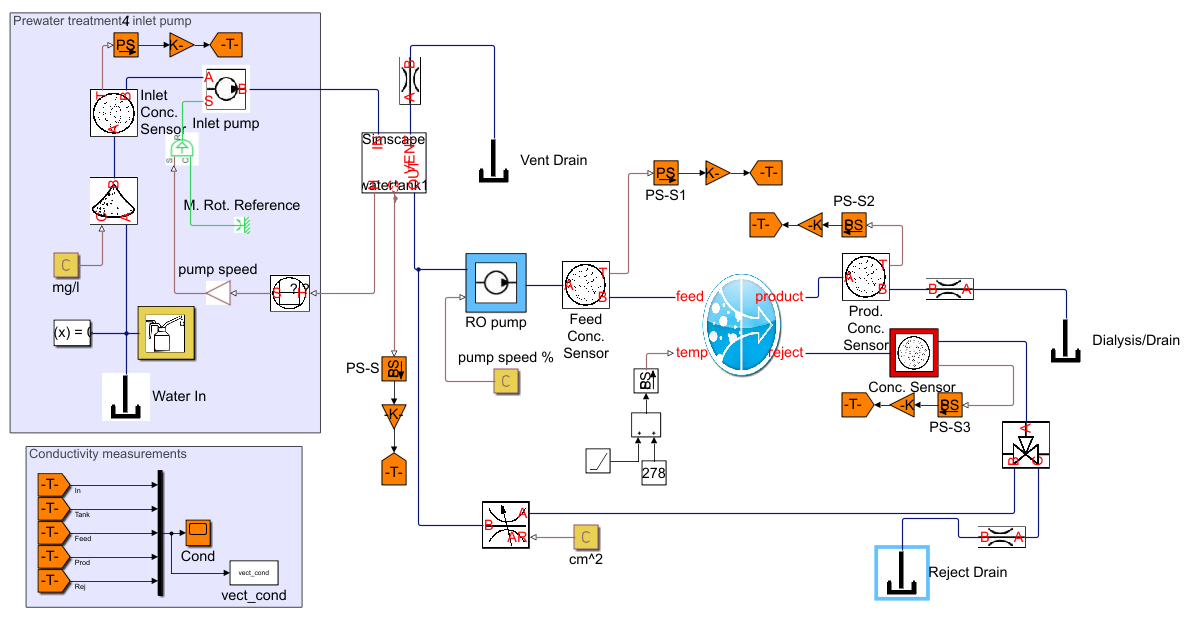
\includegraphics[width=\textwidth]{simscape_fc1.PNG}
\caption{Model made in Matlab tool Simscape}
\label{fig:simscape}
\end{figure}

\begin{figure}[h]
\centering
    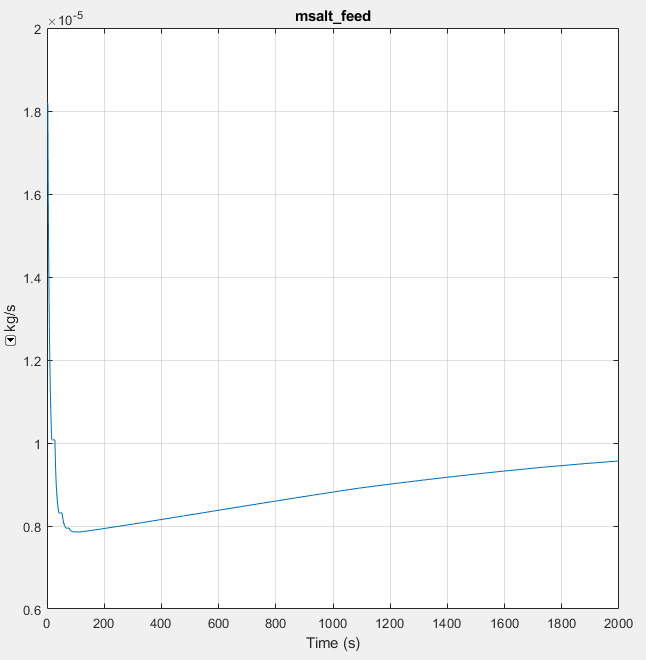
\includegraphics[width=0.5\textwidth]{msalt_feed.PNG}
    \caption{Salt concentration feedwater}
    \label{fig:msaltf}
\end{figure}

\begin{figure}[h]
\centering
  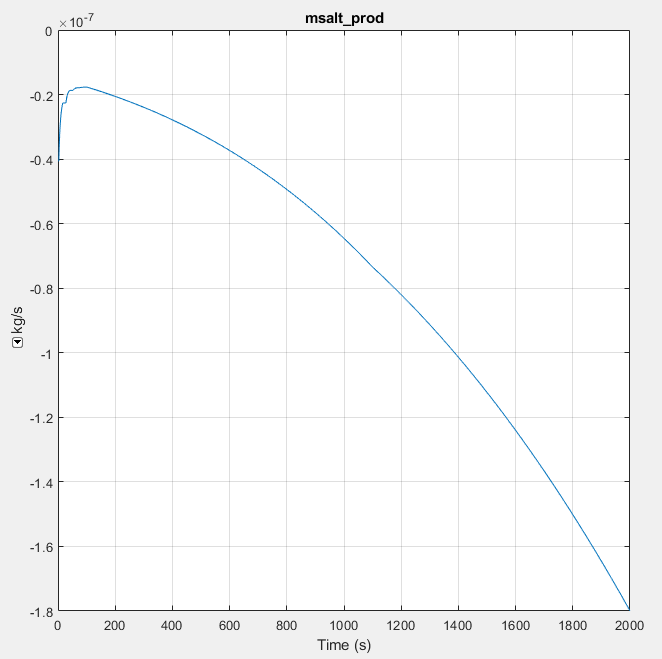
\includegraphics[width=0.5\linewidth]{msalt_prod.PNG}
  \caption{Salt concentration productwater}
  \label{fig:msalp}
\end{figure}

\begin{figure}[h]
  \centering
  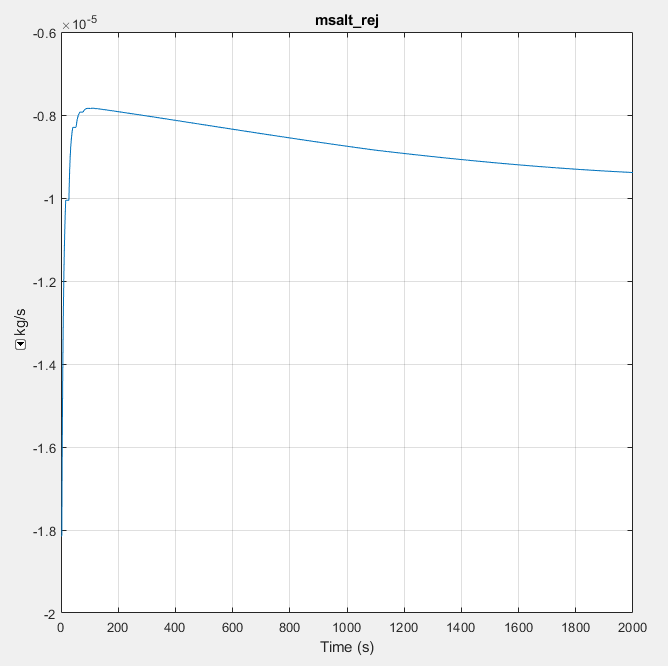
\includegraphics[width=0.5\linewidth]{msalt_rej.PNG}
  \caption{Salt concentration reject water}
  \label{fig:msaltr}
\end{figure}

\begin{figure}[h]
  \centering
  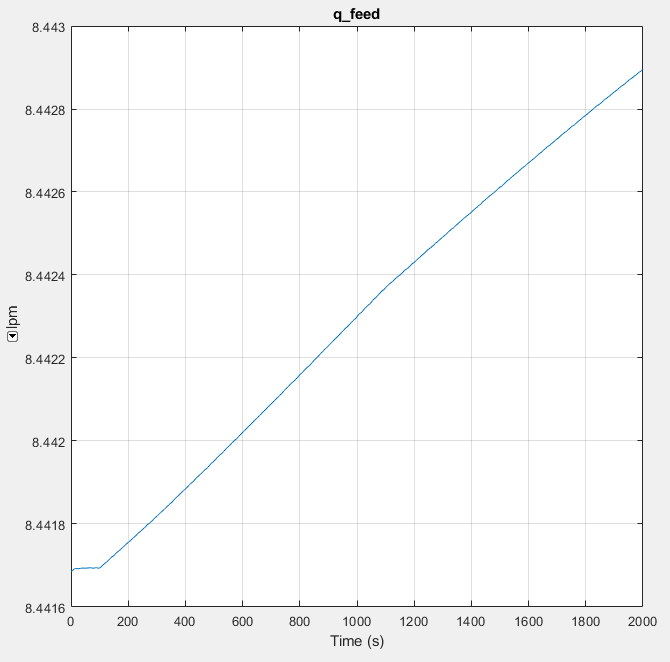
\includegraphics[width=0.5\linewidth]{q_feed.PNG}
  \caption{Flow feed side}
  \label{fig:qf}
\end{figure}

\begin{figure}[h]
  \centering
  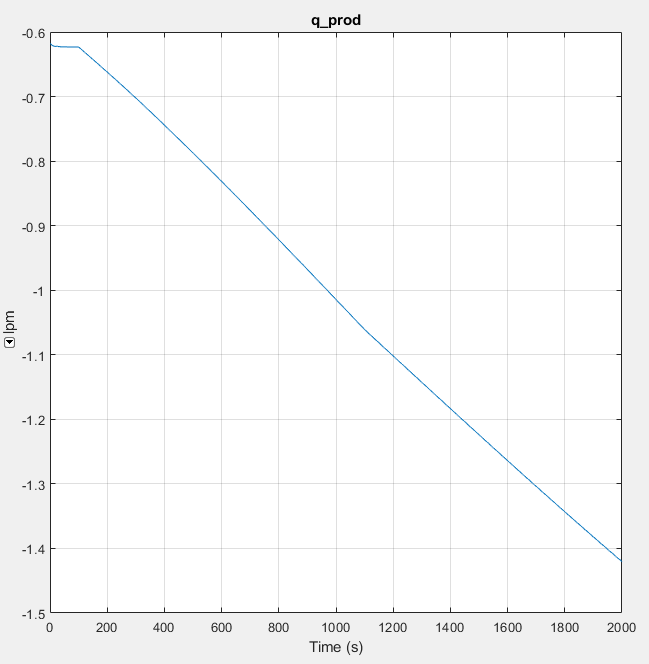
\includegraphics[width=0.5\linewidth]{q_prod.PNG}
  \caption{Flow product side}
  \label{fig:qp}
\end{figure}

\begin{figure}[h]
  \centering
  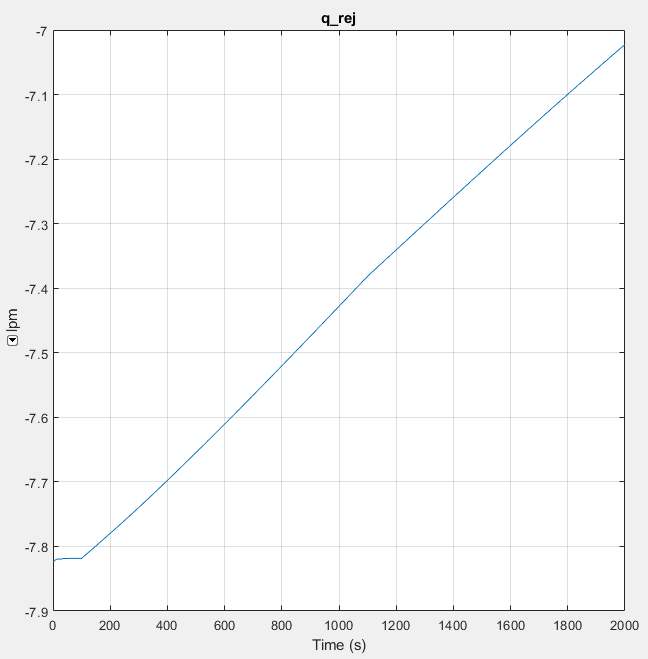
\includegraphics[width=0.5\linewidth]{q_rej.PNG}
  \caption{Flow reject side}
  \label{fig:qrej}
\end{figure}

\begin{figure}[h]
\centering
\begin{minipage}{.5\textwidth}
    \centering
    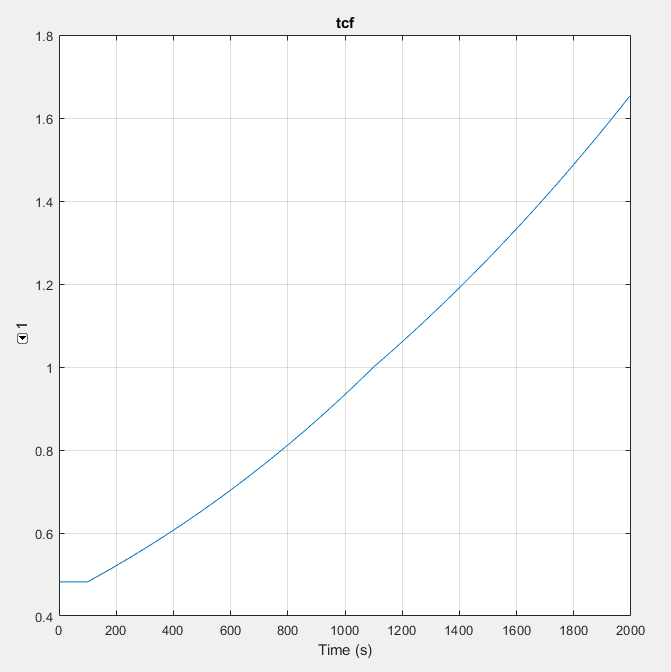
\includegraphics[width=\textwidth]{tcf.PNG}
    \caption{Temperature correction factor}
    \label{fig:tcf}
\end{minipage}
\begin{minipage}{.5\textwidth}
  \centering
  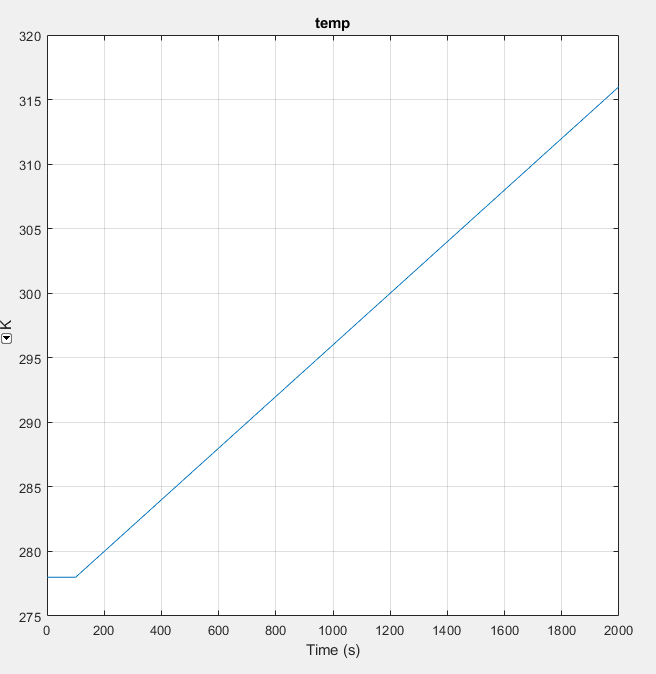
\includegraphics[width=\linewidth]{temp.PNG}
  \caption{Temperature}
  \label{fig:temp}
\end{minipage}
\end{figure}


\begin{figure}[h]
  \centering
  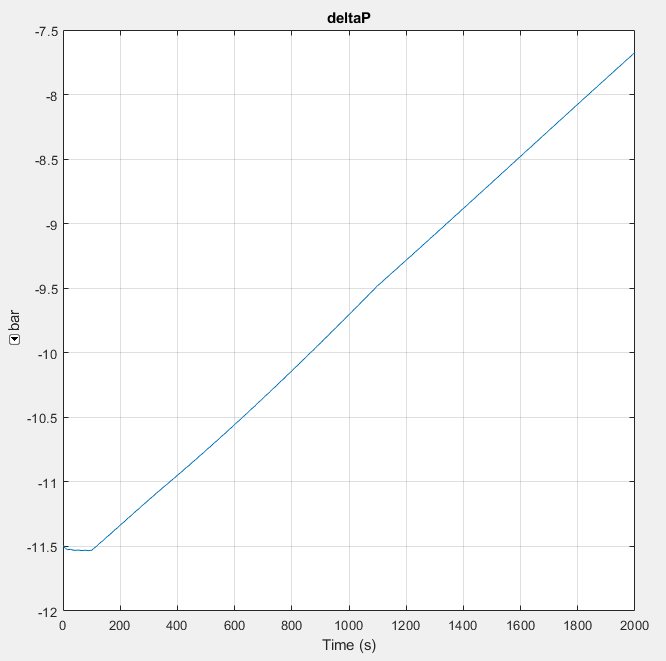
\includegraphics[width=0.5\linewidth]{deltap.PNG}
  \caption{Pressure drop feed side to product side}
  \label{fig:deltap}
\end{figure}


\begin{figure}[h]
  \centering
  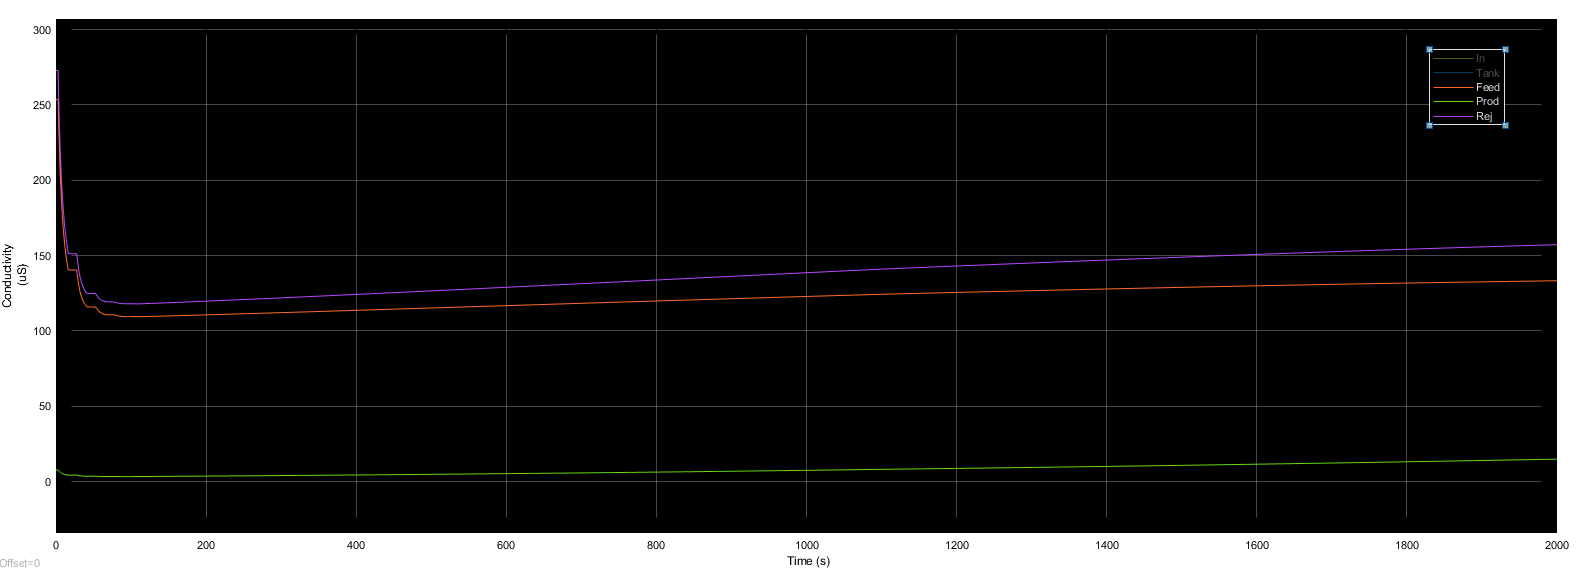
\includegraphics[width=1.1\linewidth]{cond.PNG}
  \caption{Conductivity in feed, reject and product side}
  \label{fig:cond}
\end{figure}

\newpage


\section{Flowchart investigation}
By changing the flow path in the test setup both the one pump system and two pump system could be investigated and their performance could be compared. Both Systems were considered fulfilling most of the requirements, section \ref{framing}, for an updated version. \\

One pump system, figure \ref{fig:FlowCInves1}, The one pump system was designed to use both a tank and the recirculation loop as a water source and to create pressure by generating a large flow over the membrane and recirculation restrictor. \\


Two pump system, figure \ref{fig:Sys2}, In the two pump system the water path was modified so that the feed pump only used a tank as a source and pressureized the entire recirculation loop. The recirculation pump was used to recirculate the already\\ pressureized water within the recirculation loop.\\


An overview of the systems can be seen below.\\
\begin{figure}[h]
\centering
\begin{minipage}{.5\textwidth}
    \centering
    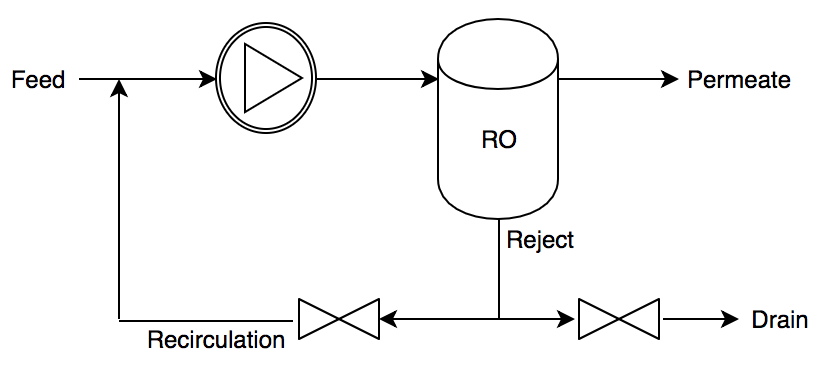
\includegraphics[width=0.8\textwidth]{Sys1}
    \caption{One pump system}
    \label{fig:System1}
\end{minipage}%
\begin{minipage}{.5\textwidth}
  \centering
  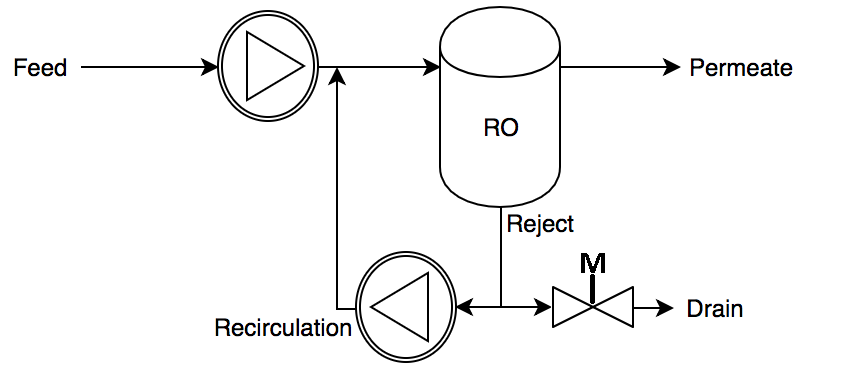
\includegraphics[width=.8\linewidth]{Sys2}
  \caption{Two pump system}
  \label{fig:System2}
\end{minipage}
\end{figure}

\newpage

\section{Investigation}

In order to compare the two systems and understand how the membrane performed in different working conditions both systems needed to be tested. The tests were conducted by controlling the temperature, pumps and the conductivity in the recirculation loop and log how the different conditions affected the system and the membrane. 

The tests were conducted by changing the temperature, recirculation conductivity and pump speed and meassure how the system behaved once it had reached steady state. The tests were divided into three test sequences. One test sequence was performed with room temperatured water (19 C), one with water heated to 30 C and in the last test sequence the water was heated to 40 C. Every test sequence included data from 8 steady state points with different settings on feed conductivity and pump speed. The test sequences are displayed in the table below. 

\begin{table}[h]
\centering
\begin{tabular}{|p{1.4cm}||p{2cm}|p{3.2cm}|p{1.8cm}|}
 \hline
 \textbf{Steady state }&Temperature&Feed Conductivity&Motor effect \\
 \hline
 1.1 & 18 $^\circ$C   & 280 \SI{}{\micro\siemens} & 60 \% \\
 1.2   &  18 $^\circ$C   & 500 \SI{}{\micro\siemens} & 60 \% \\
 1.3 &  18 $^\circ$C  &1000 \SI{}{\micro\siemens} & 60 \% \\
 1.4 &  18 $^\circ$C  &1000 \SI{}{\micro\siemens} & \textbf{80 \%} \\
 1.5 &18 $^\circ$C &2000 \SI{}{\micro\siemens}& 60 \%\\
 1.6 &18 $^\circ$C  &2000 \SI{}{\micro\siemens}& \textbf{80 \%}\\
 1.7   &18 $^\circ$C & 3000 \SI{}{\micro\siemens}&60 \% \\
 1.8   &18 $^\circ$C&3000 \SI{}{\micro\siemens}& \textbf{80 \%}\\
 \hline
 2.1 & 30 $^\circ$C & 280 \SI{}{\micro\siemens}&60 \%\\
 2.2 & 30 $^\circ$C &500 \SI{}{\micro\siemens}& 60 \%\\
 2.3 & 30 $^\circ$C&1000 \SI{}{\micro\siemens}& 60 \%\\
 2.4 & 30 $^\circ$C&1000 \SI{}{\micro\siemens}& \textbf{80 \%}\\
 2.5 & 30 $^\circ$C&2000 \SI{}{\micro\siemens}& 60 \%\\
 2.6 & 30 $^\circ$C&2000 \SI{}{\micro\siemens}& \textbf{80 \%}\\
 2.7 & 30 $^\circ$C& 3000 \SI{}{\micro\siemens}&60 \%\\
 2.8 & 30 $^\circ$C& 3000 \SI{}{\micro\siemens}&\textbf{80 \%}\\
 \hline 
 3.1 & 40 $^\circ$C& 280 \SI{}{\micro\siemens}& 60 \%\\
 3.2 & 40 $^\circ$C &500 \SI{}{\micro\siemens}& 60 \%\\
 3.3 & 40 $^\circ$C  & 1000 \SI{}{\micro\siemens}& 60 \%\\
 3.4 & 40 $^\circ$C  & 1000 \SI{}{\micro\siemens}& \textbf{80 \%}\\
 3.5 & 40 $^\circ$C&2000 \SI{}{\micro\siemens}& 60 \%\\
 3.6 & 40 $^\circ$C &2000 \SI{}{\micro\siemens}& \textbf{80 \%}\\
 3.7 & 40$^\circ$C &3000 \SI{}{\micro\siemens}& 60 \%\\
 3.8 & 40$^\circ$C &3000 \SI{}{\micro\siemens}& \textbf{80 \%}\\
\hline
\end{tabular}
\caption{Testcases}
    \label{tab:test cases} 
\end{table}


\subsection{Current system, Test sequence 1, part 1}

The water in the tank was heated while the test was running. Because of this, the test was split up in two parts, first the motor was set to 60\% and steady state 1.1, 1.2, 1.3, 1.5 and 1.7 were investigated. In the part 2, the motor was set to 80 \% and steady state 1.4, 1.6 and 1.8 were investigated. 
\begin{figure}[H]
    \centering
    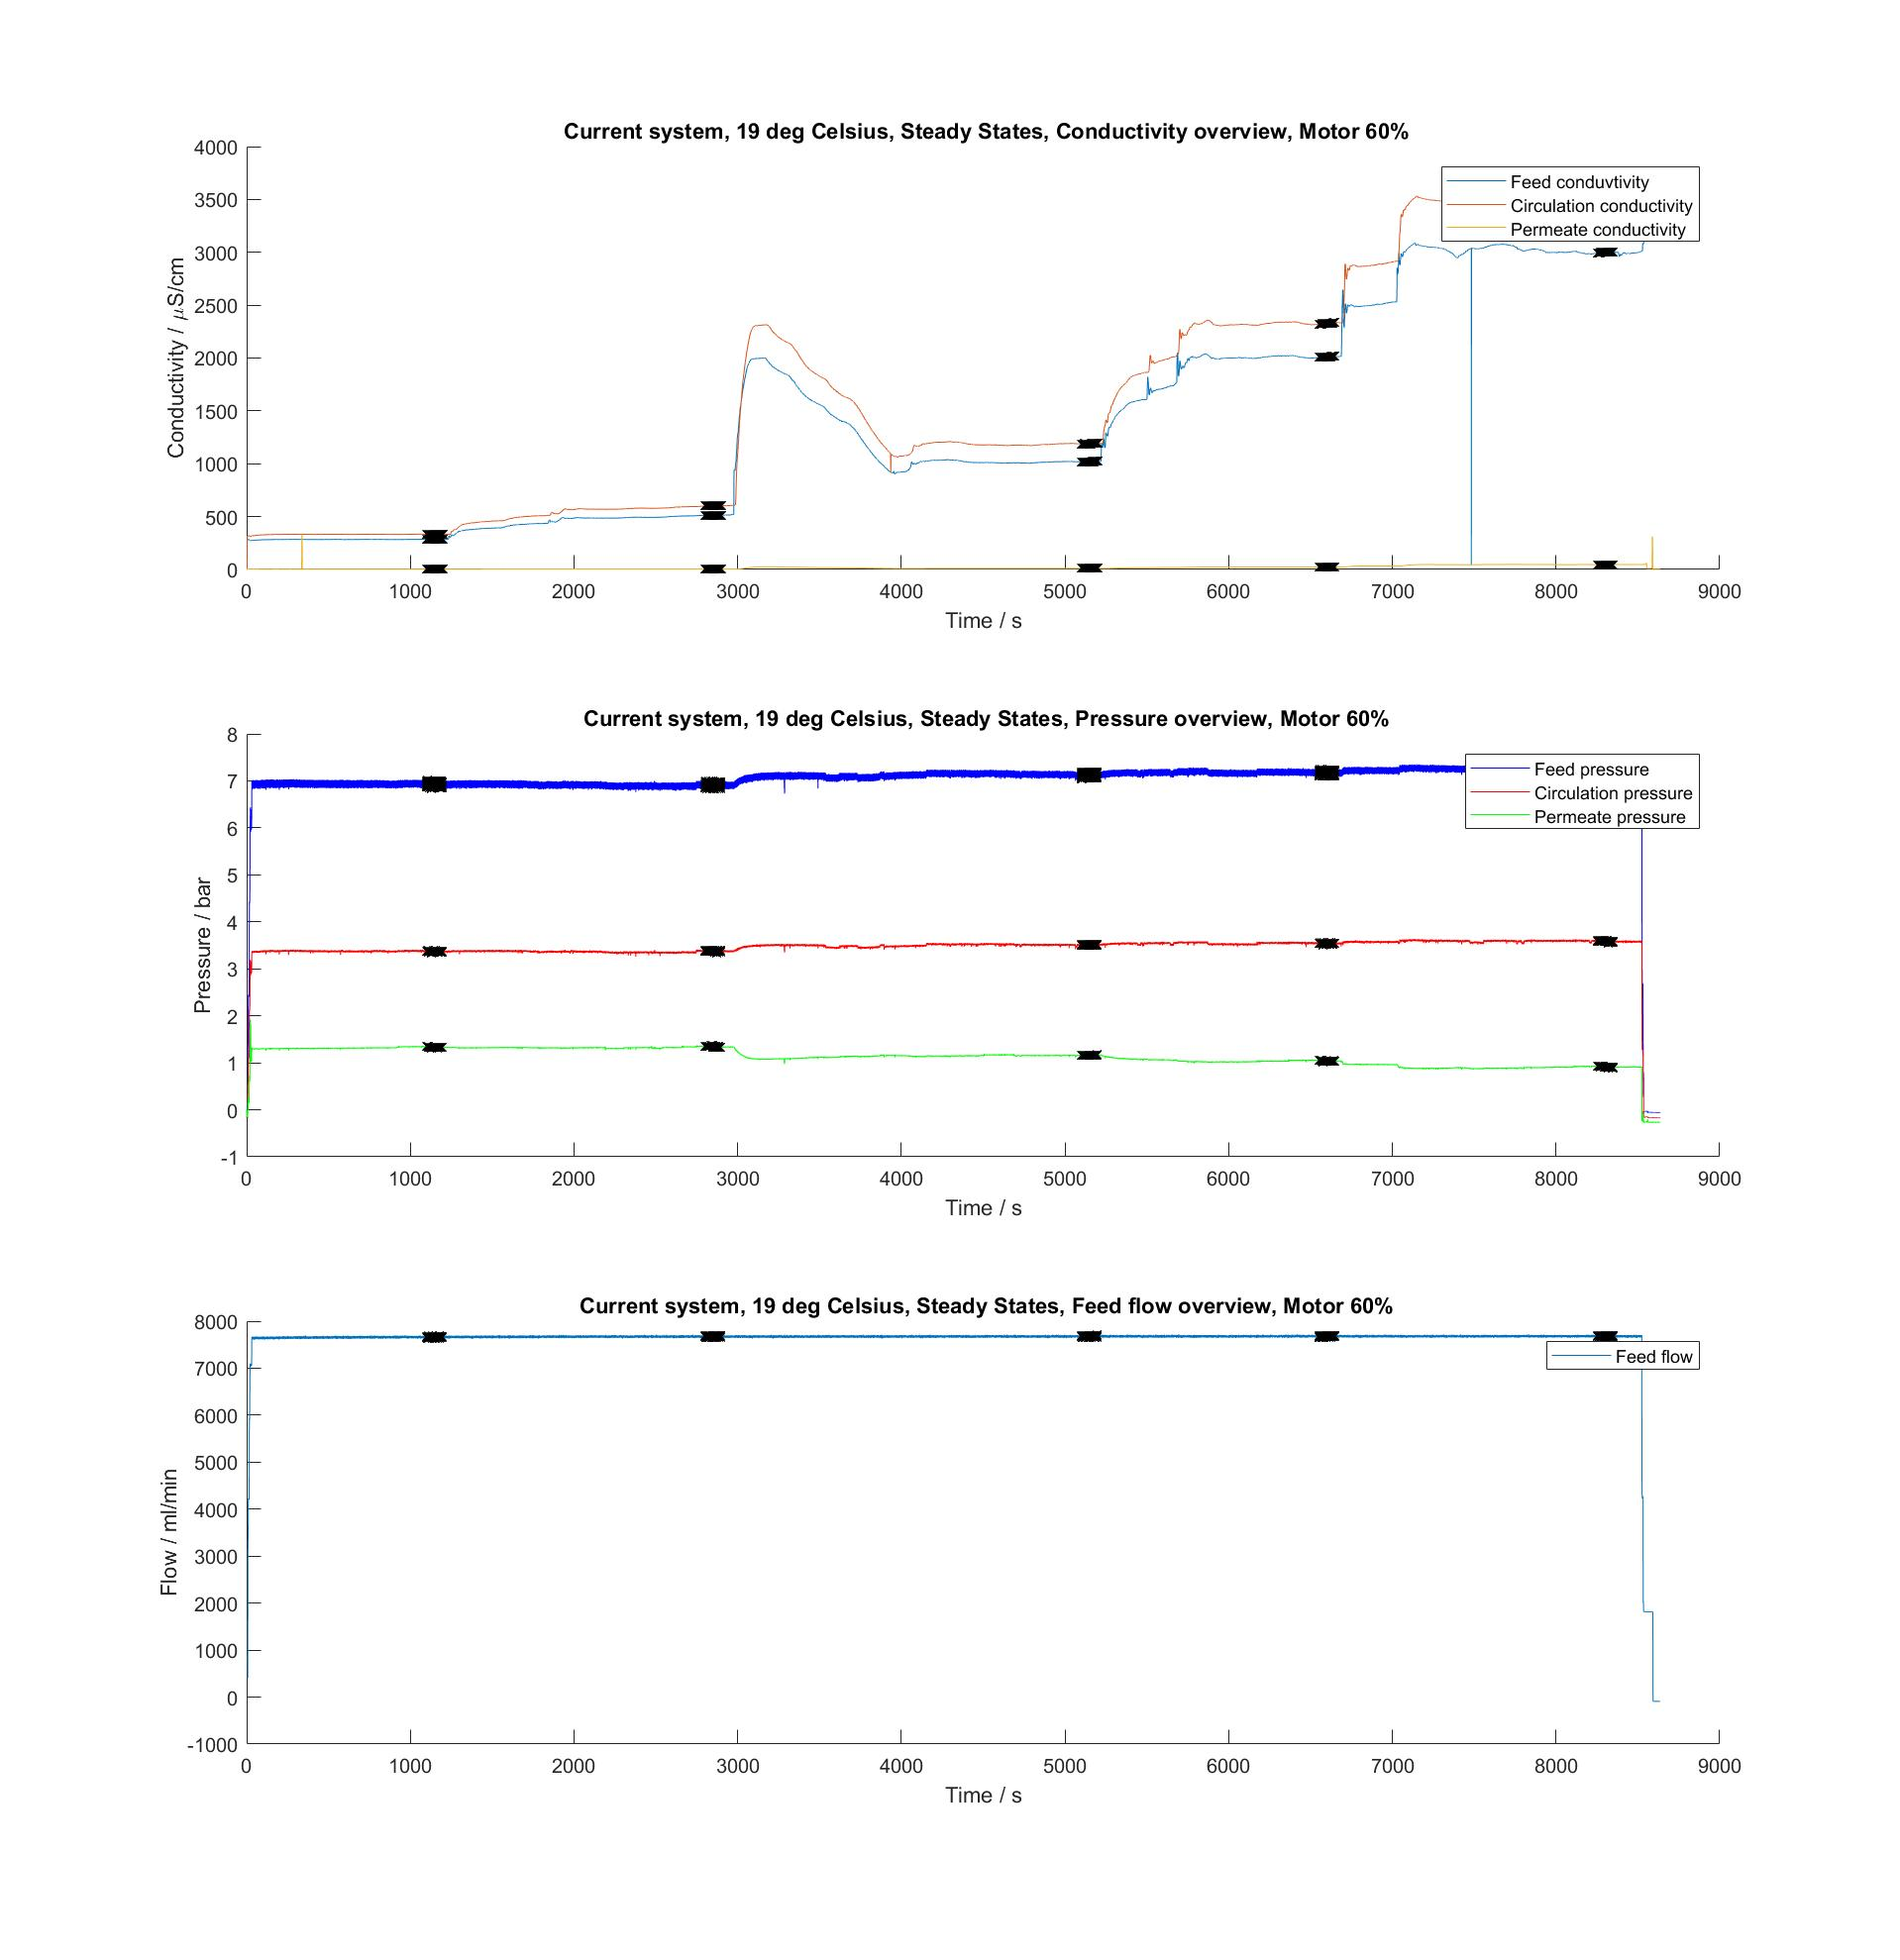
\includegraphics[width=1.1\textwidth]{overview20_60}
    \caption{Test 1, Current system, 18 degrees celsius. Steady states 1.1, 1.2, 1.3, 1.5 and 1.7 }
    \label{fig:PressConn}
\end{figure}

\newpage

\subsection{Current system, Test sequence 1, part 2}
  
\begin{figure}[H]
    \centering
    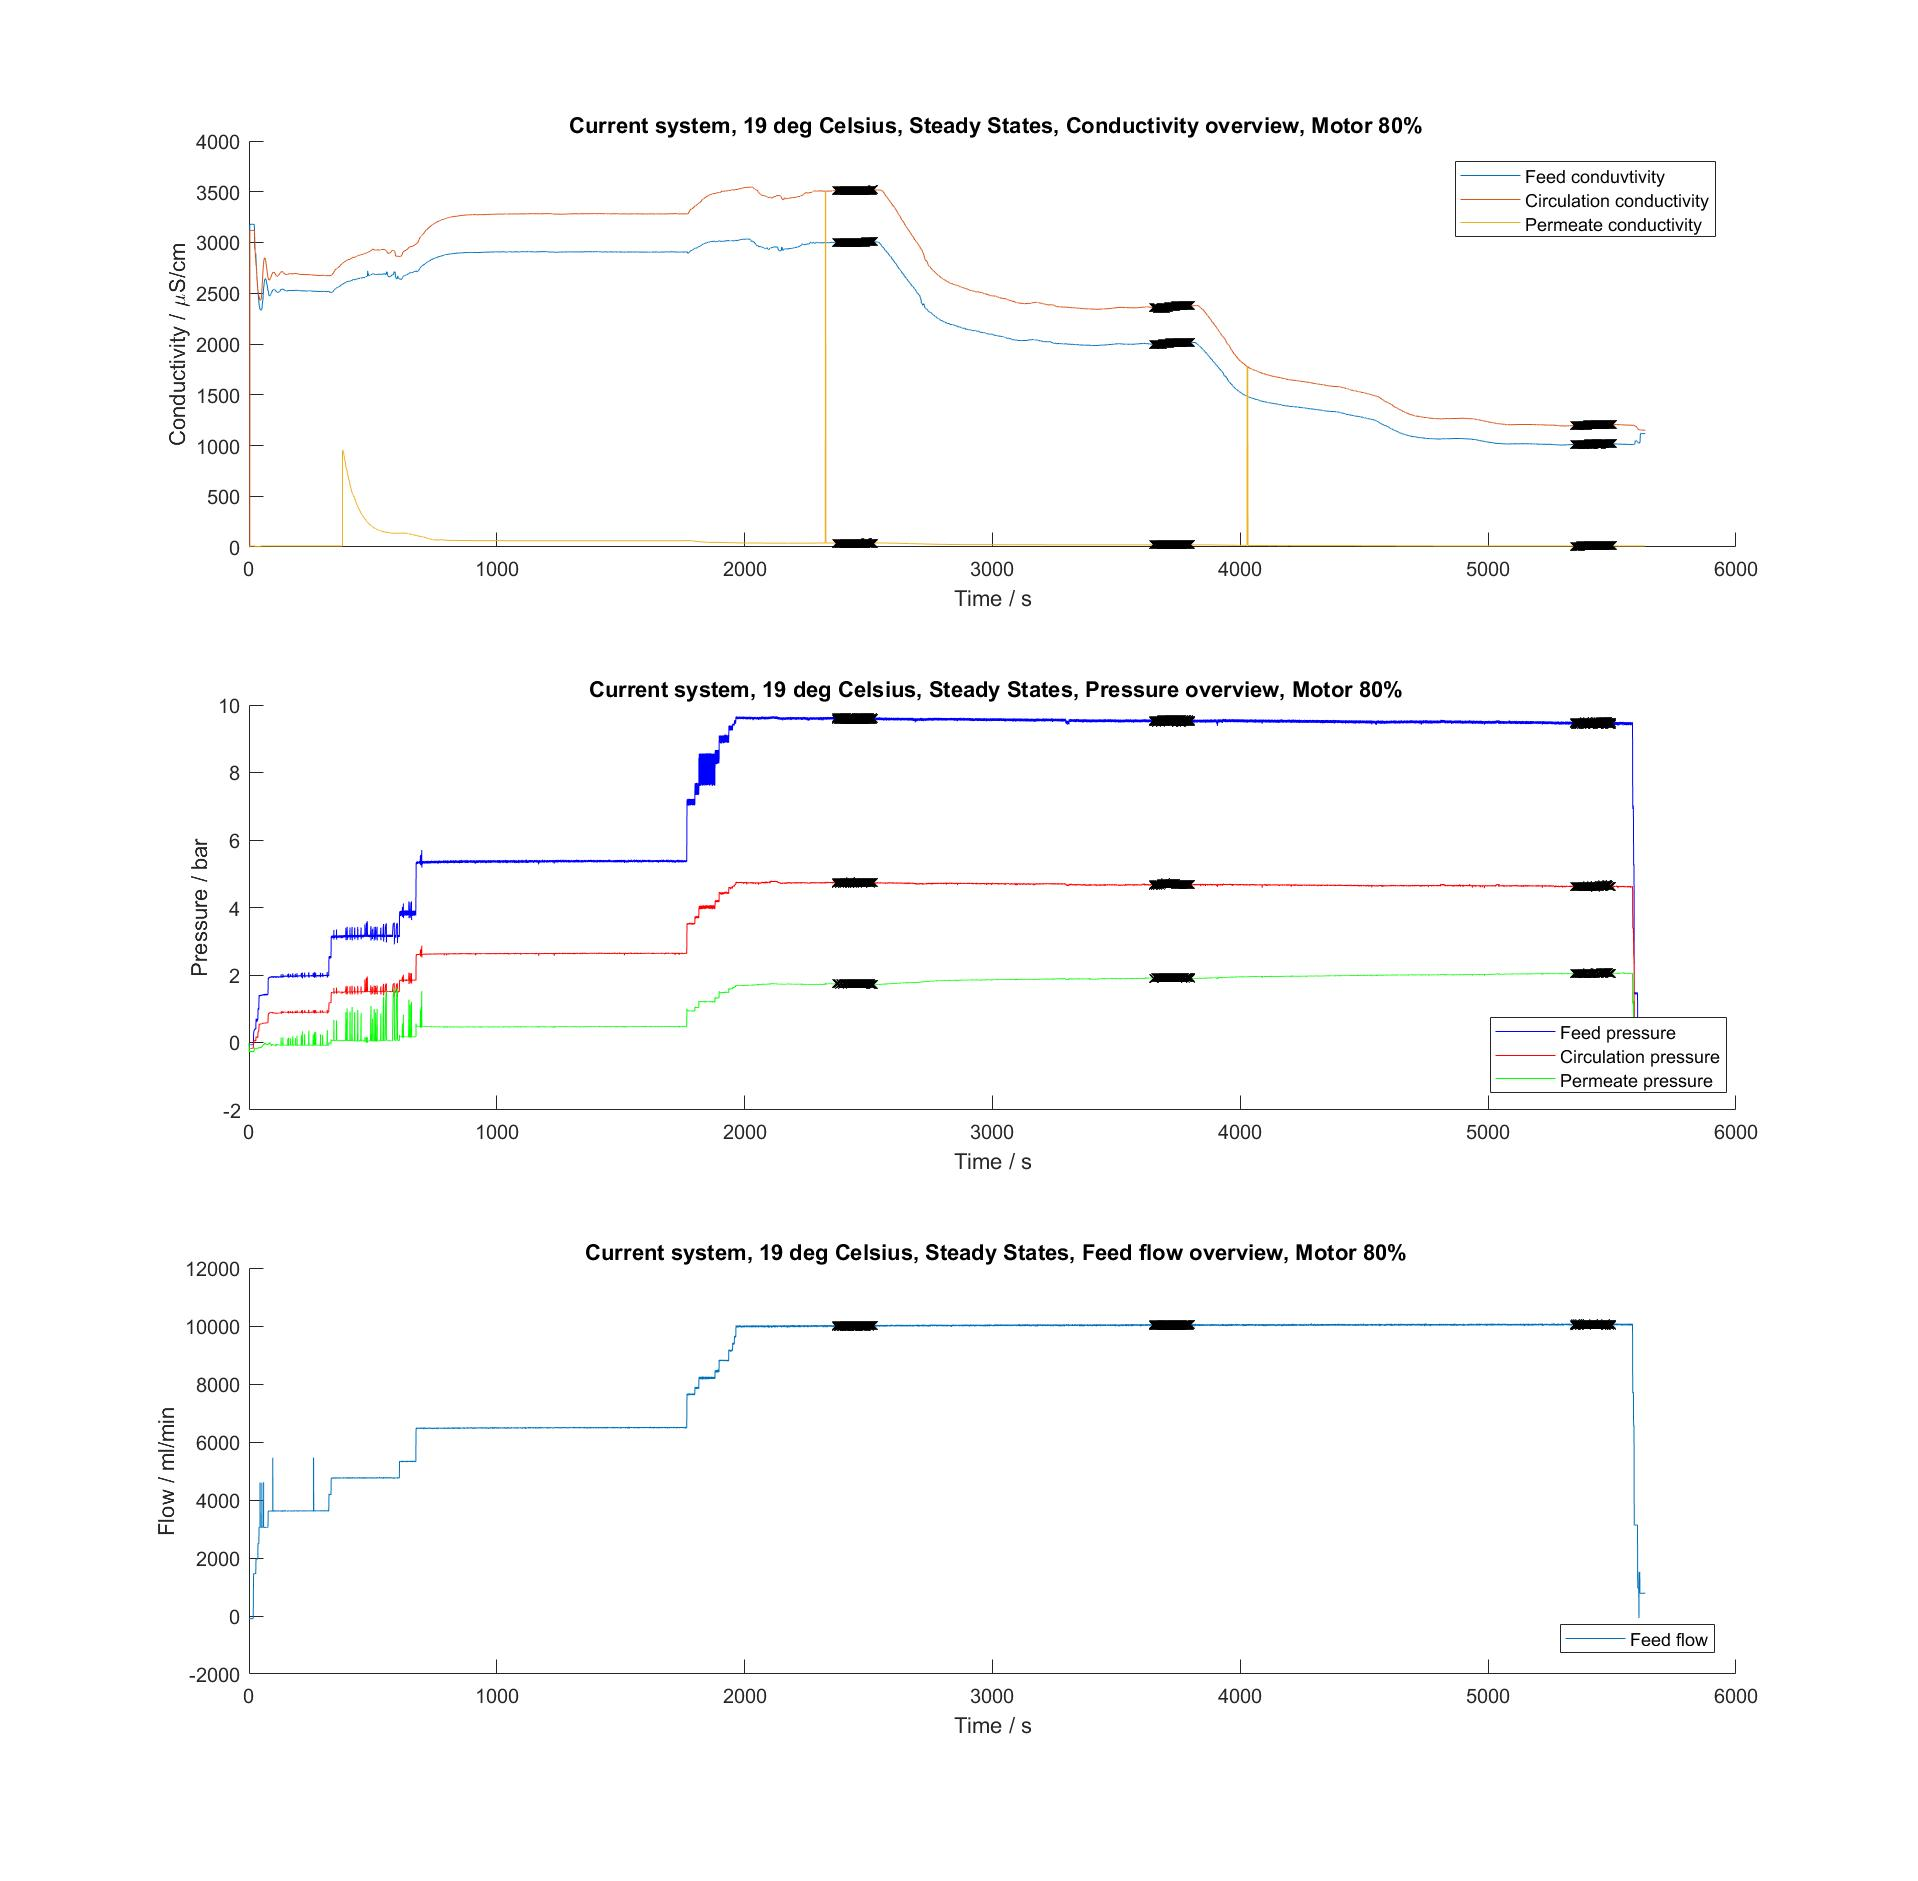
\includegraphics[width=1.1\textwidth]{overview20_80}
    \caption{Test 1, Current system, 18 degrees celsius. Steady states 1.4, 1.6 and 1.8}
    \label{fig:PressConn}
\end{figure}

\newpage

By post-procesing the data from test one in Matlab it was possible to visually show how the system parameters were affected by the changed pump speed and feed conductivity. 


insert table, results on how the different graphs changed!!!

\begin{figure}[H]
    \centering
    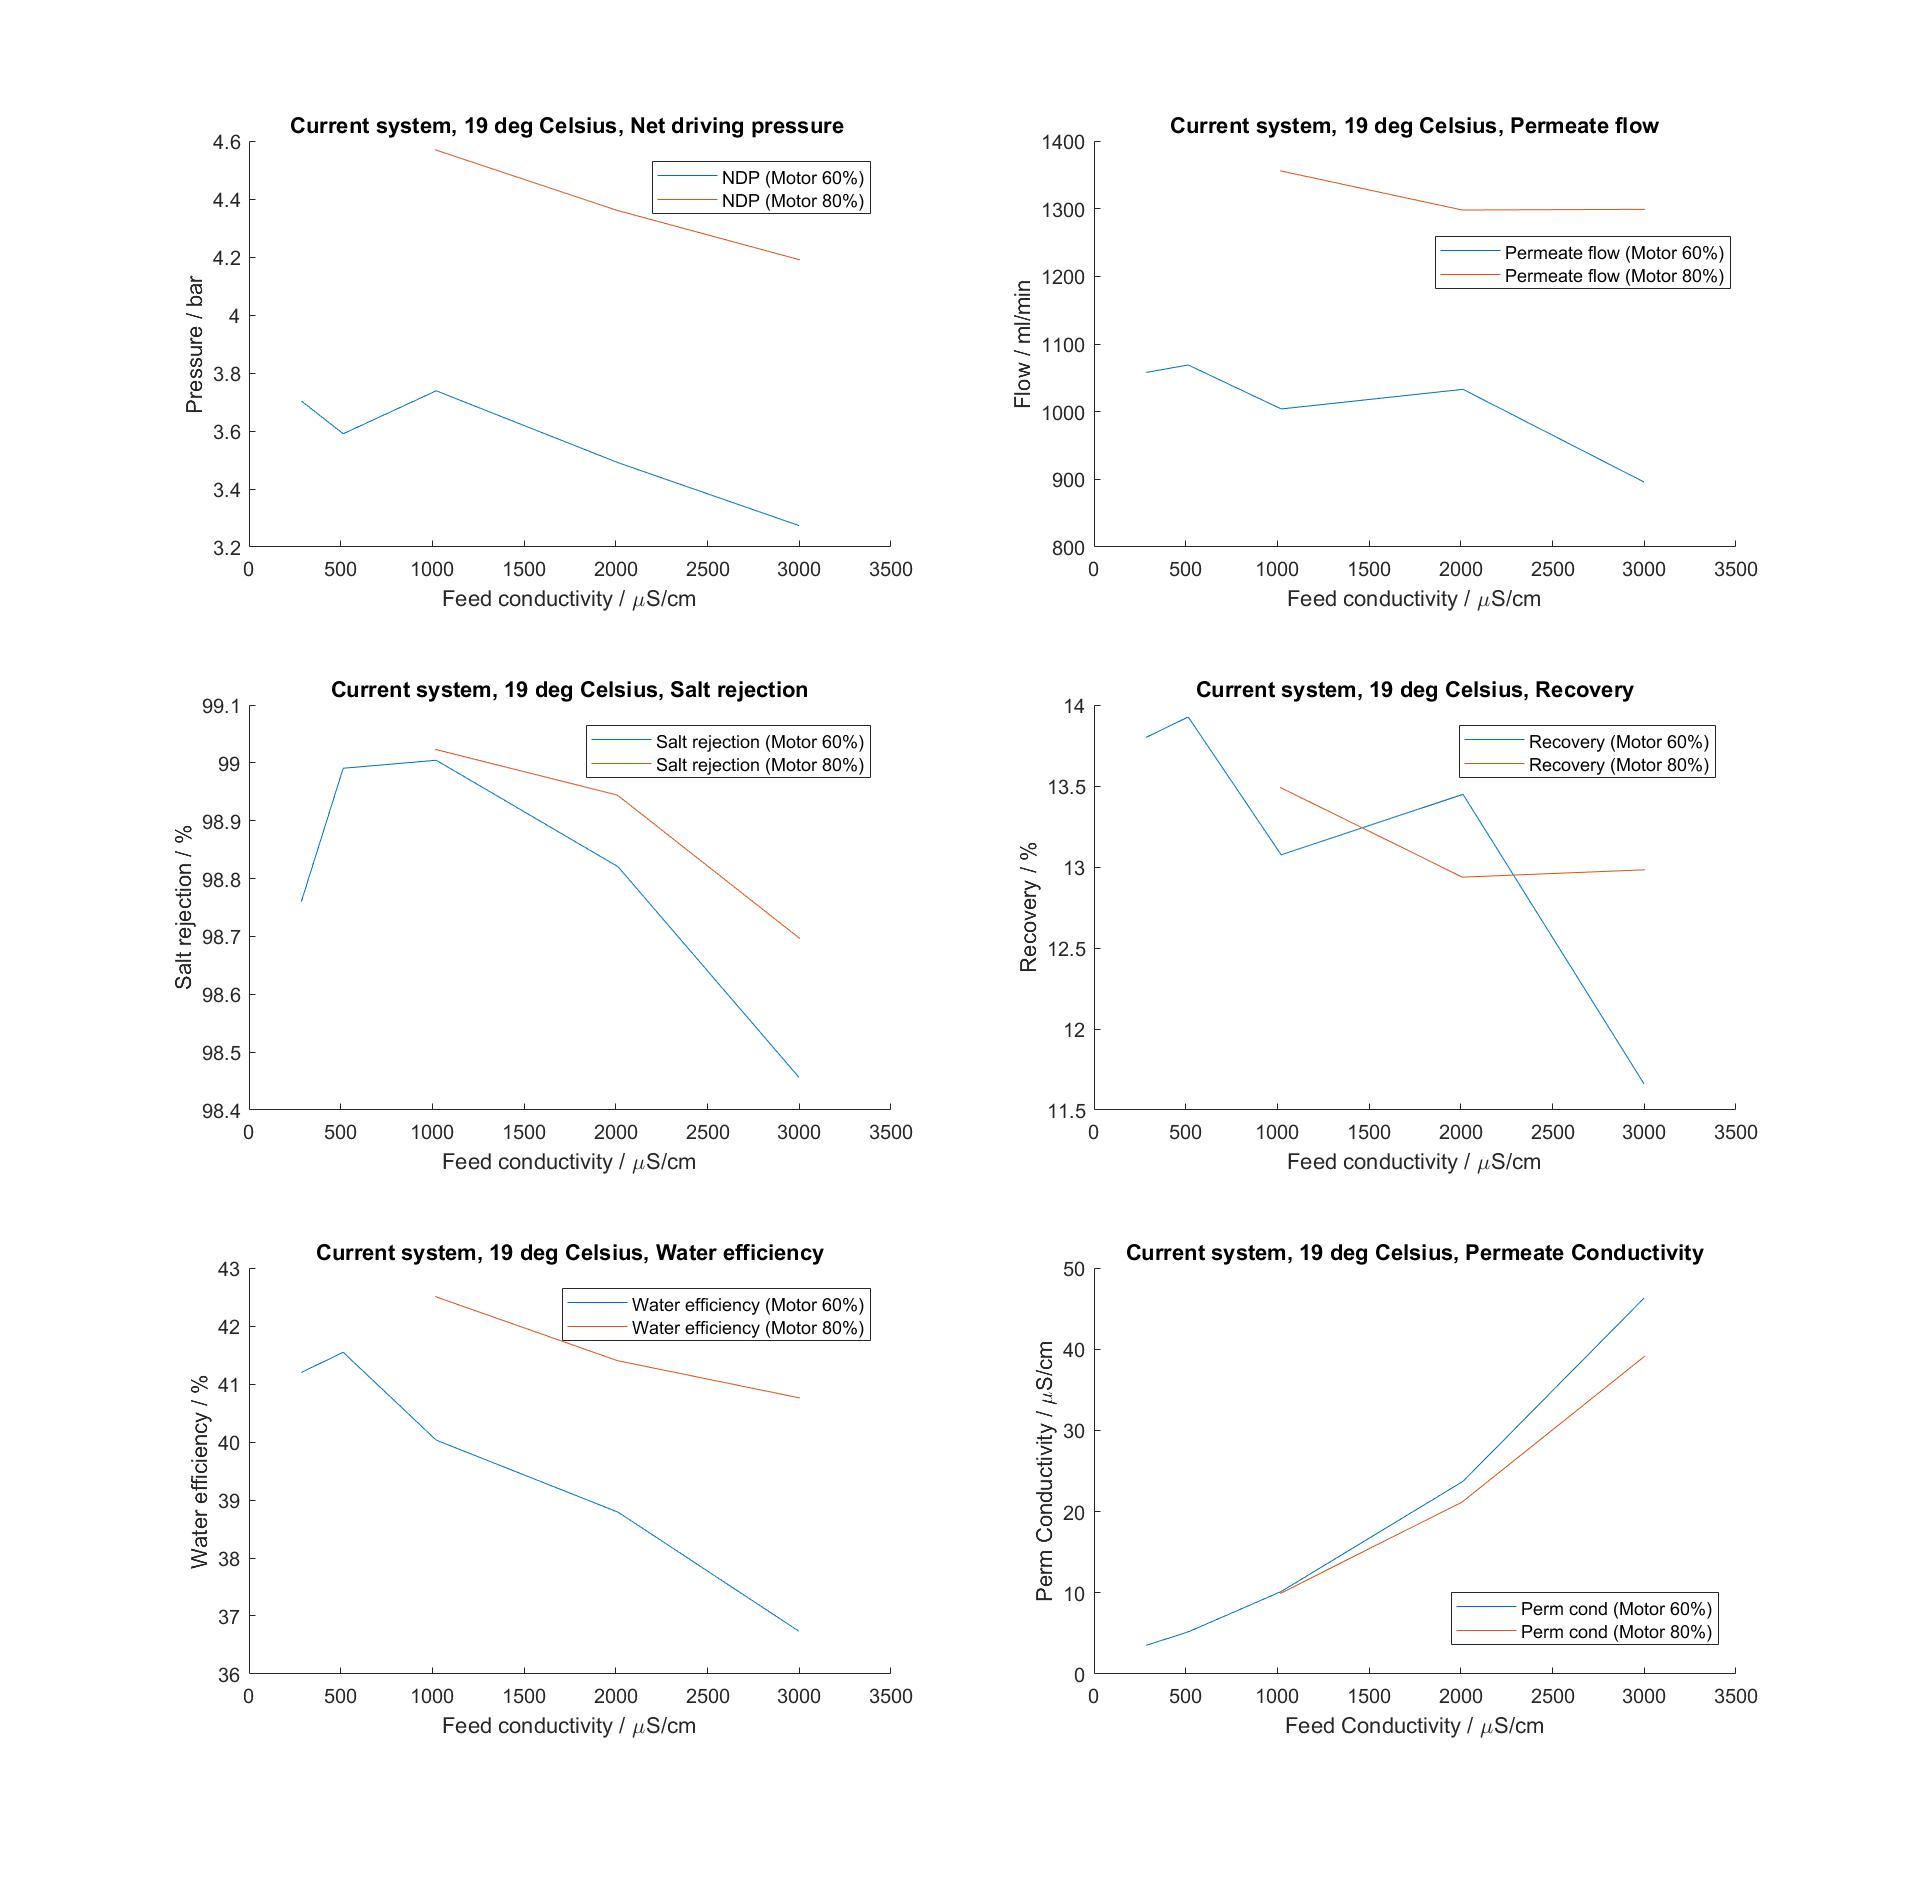
\includegraphics[width=1.1\textwidth]{Key20}
    \caption{Connections Pressure sensors}
    \label{fig:PressConn}
\end{figure}

\newpage

\subsection{Current system, Test sequence 2}

The second test was carried out by setting the heater bath to 30 degrees celsius and and adjusting the conductivity and pump speed according to the test plan. Since the water was much warmer than the air in the room, the heating caused by the pump was not as prominent and allowed all steady states to be examined in one contimous test.

\begin{figure}[H]
    \centering
    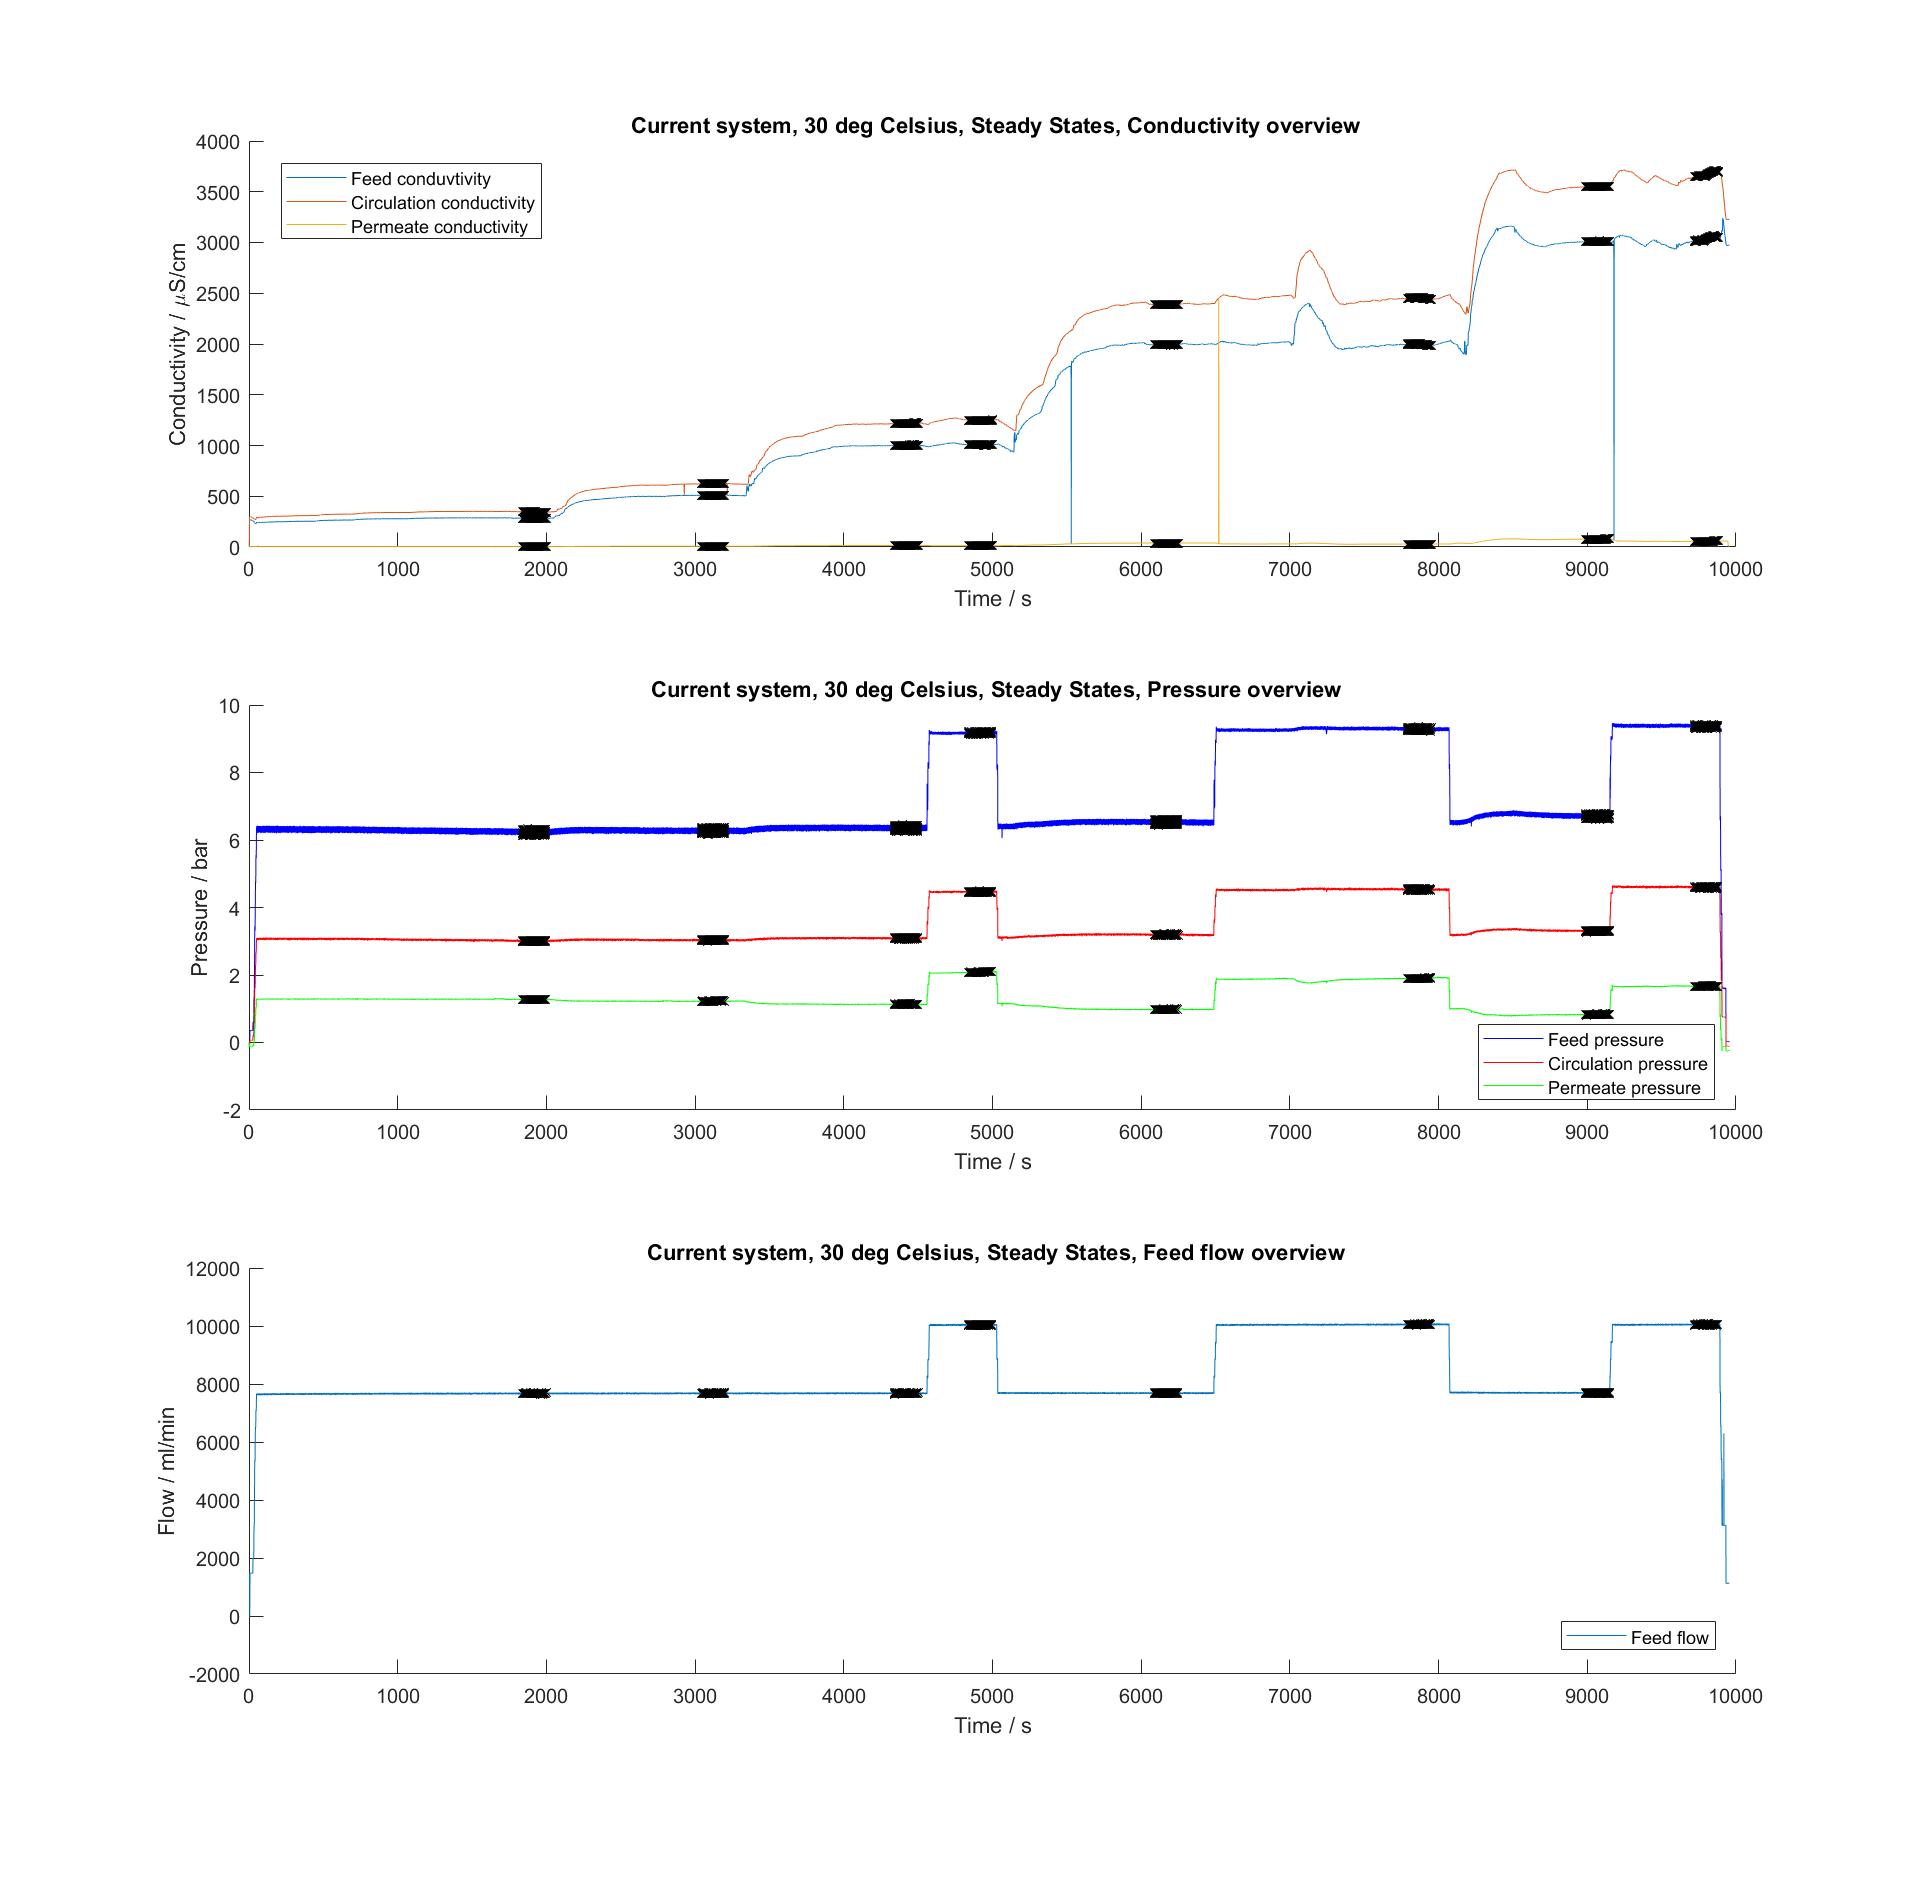
\includegraphics[width=1.1\textwidth]{overview30}
    \caption{Test 2, Current system, 30 degrees celsius. Steady states 1.1, 1.2, 1.3, 1.4 1.5, 1.6, 1.7 and 1.8}
    \label{fig:PressConn}
\end{figure}

\newpage



The data from the test was post proccesed in Matlab in exactly the same way as the previous test.

\begin{figure}[H]
    \centering
    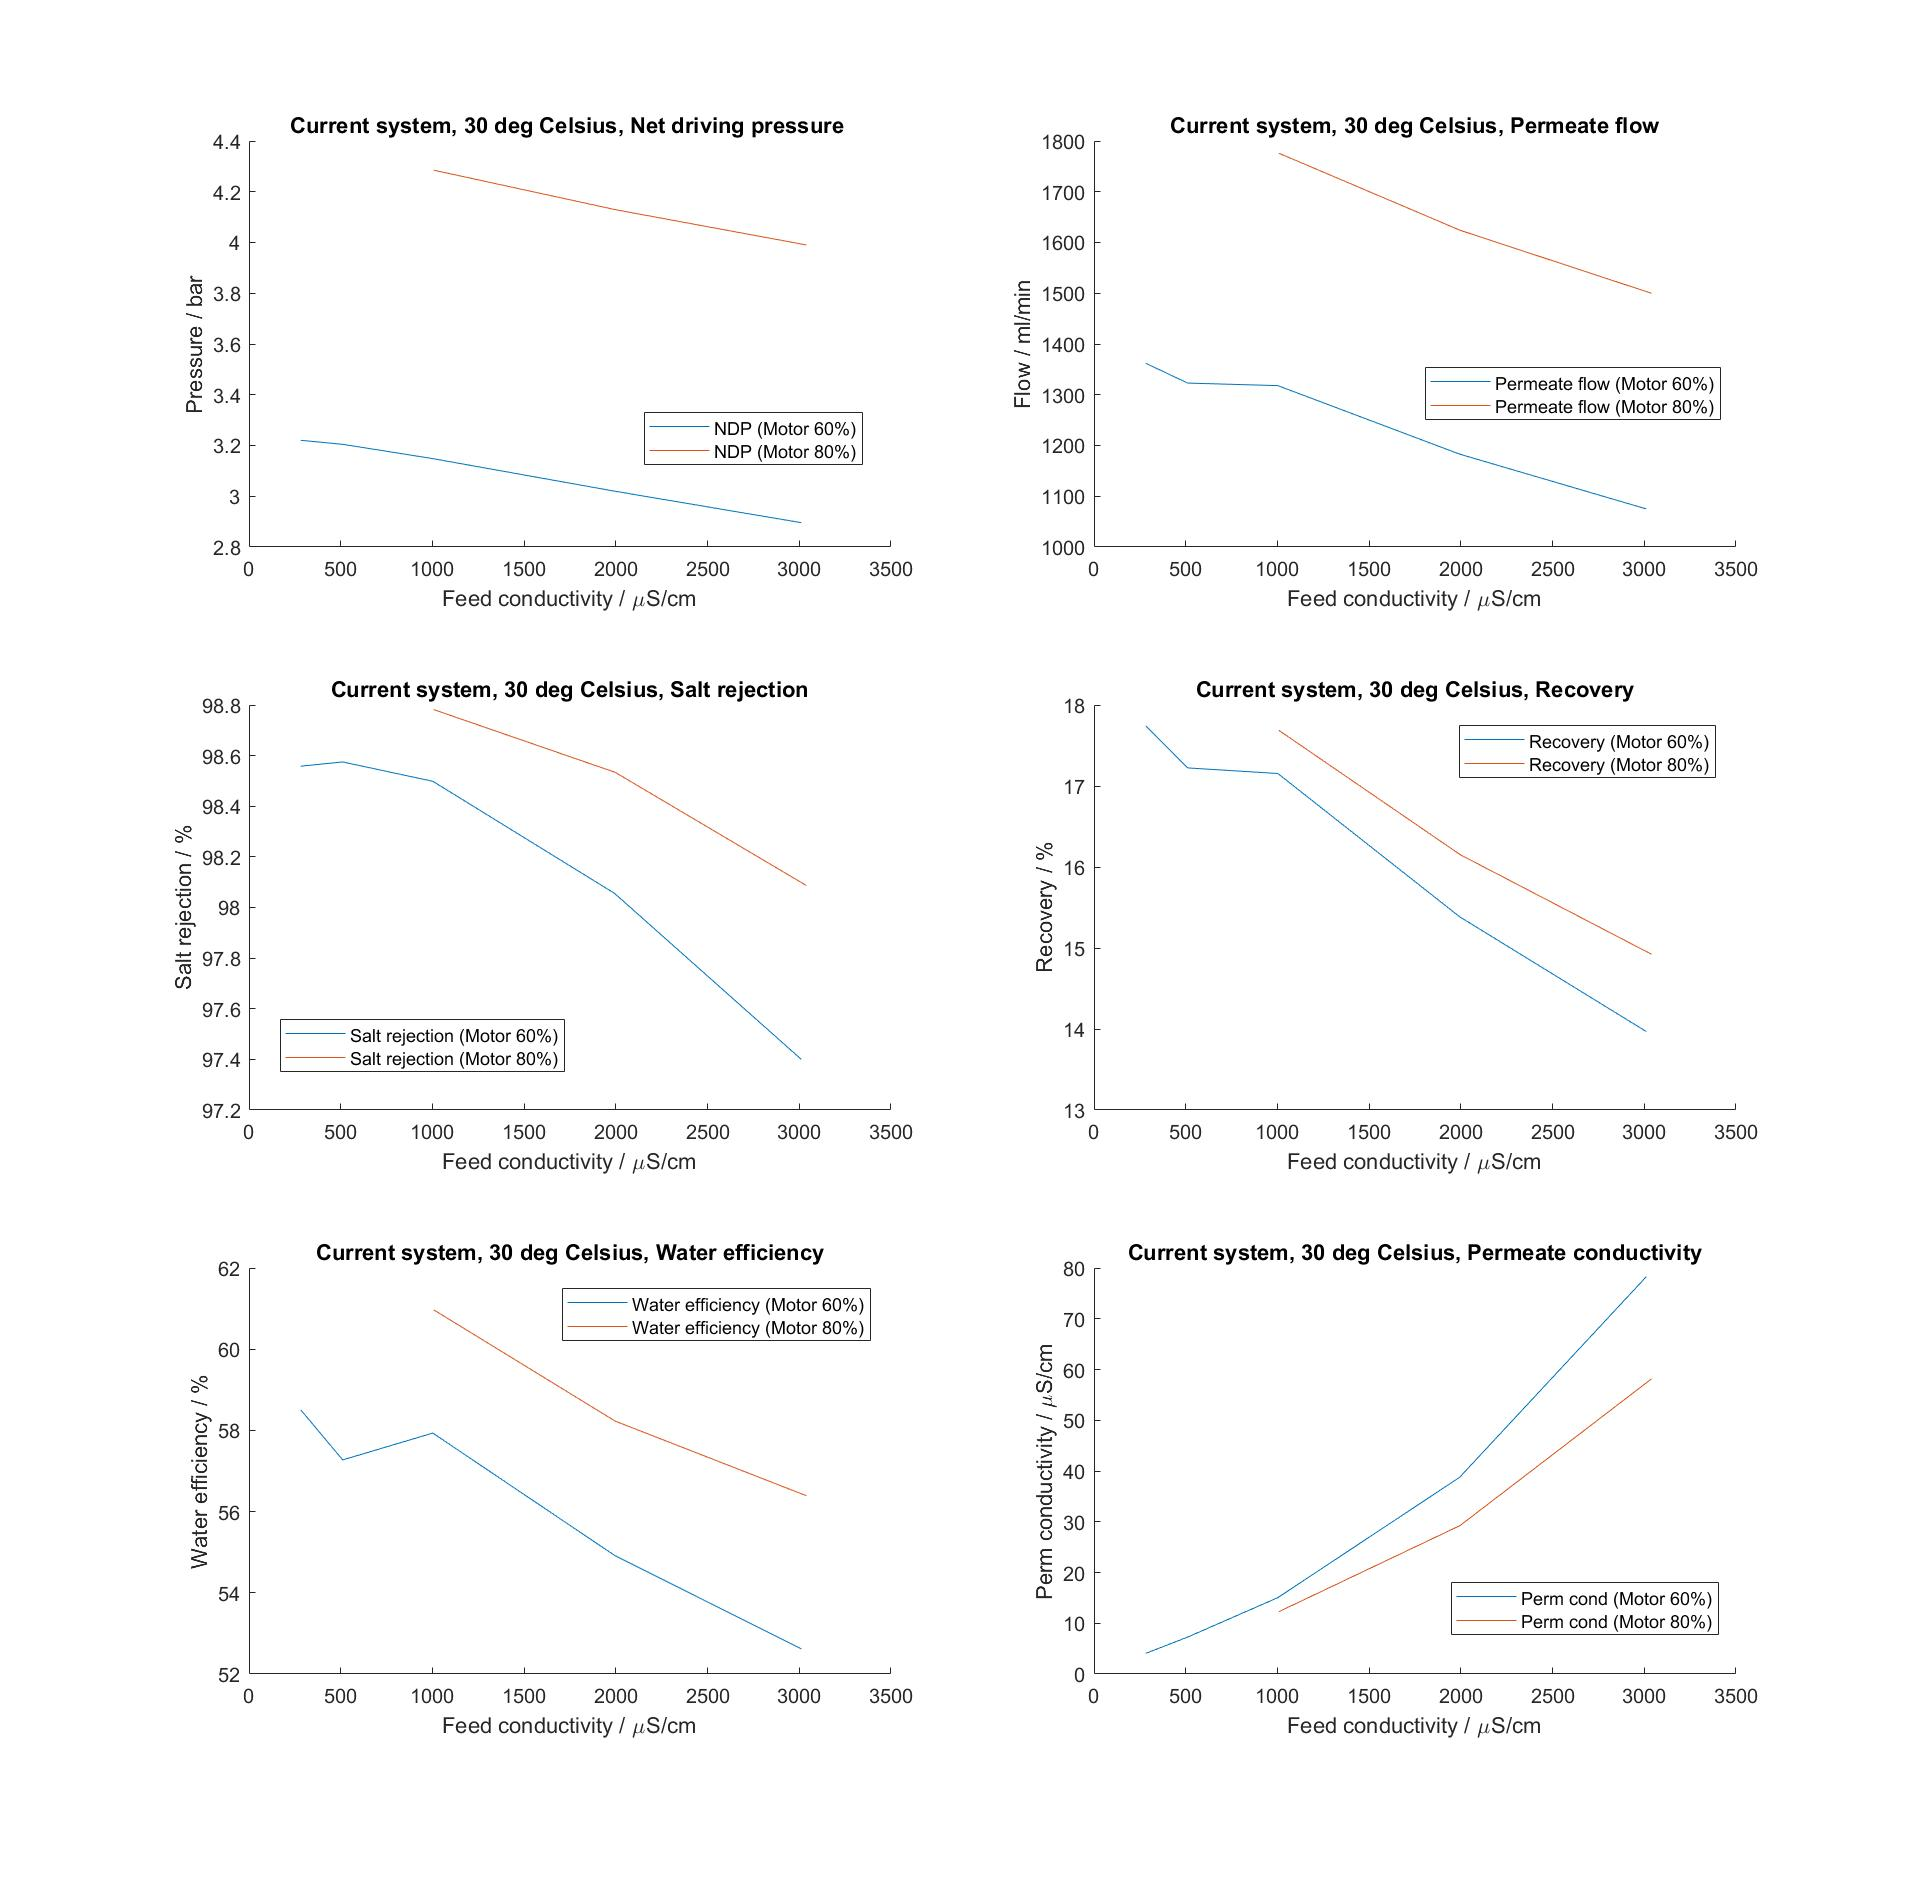
\includegraphics[width=1.1\textwidth]{Key30}
    \caption{Connections Pressure sensors}
    \label{fig:PressConn}
\end{figure}

\newpage

\subsection{Current system, Test sequence 3}

Finally the heating bath was set to 40 C and the test sequence was performed just like test sequence 2. 

\begin{figure}[H]
    \centering
    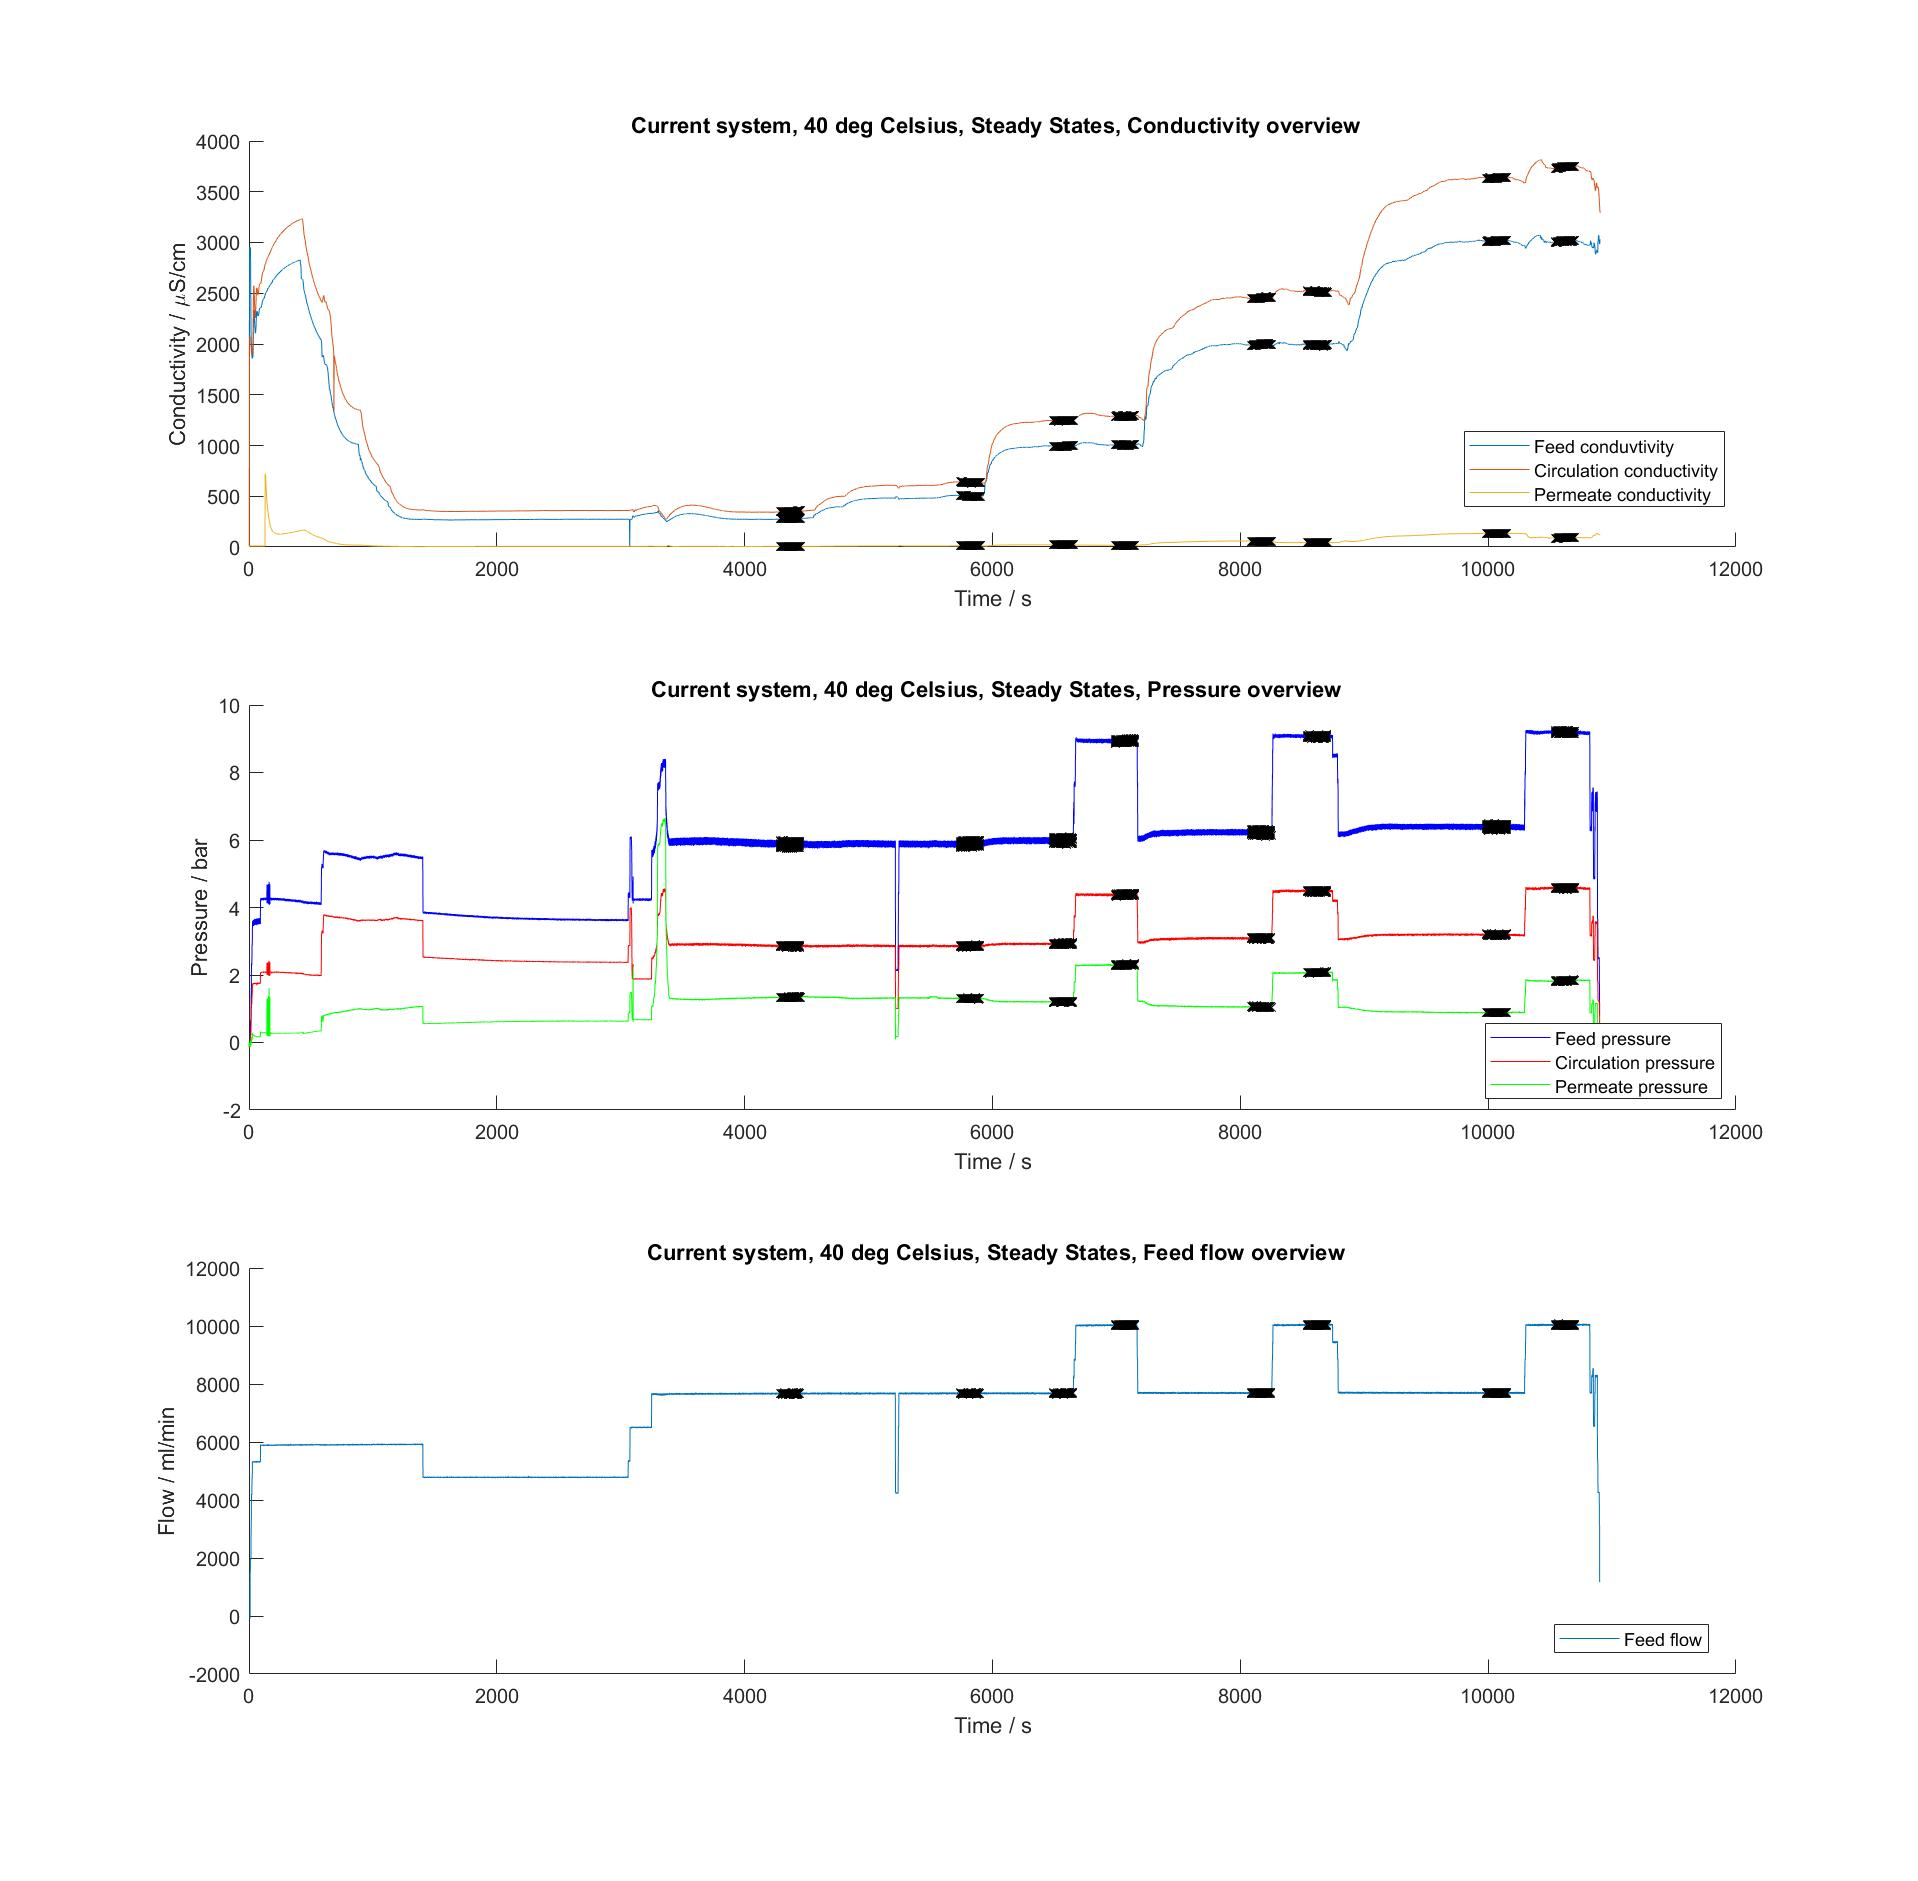
\includegraphics[width=1.1\textwidth]{overview40}
    \caption{Connections Pressure sensors}
    \label{fig:PressConn}
\end{figure}

\newpage

Post processing in matlab generated the following data from the steady states.

\begin{figure}[H]
    \centering
    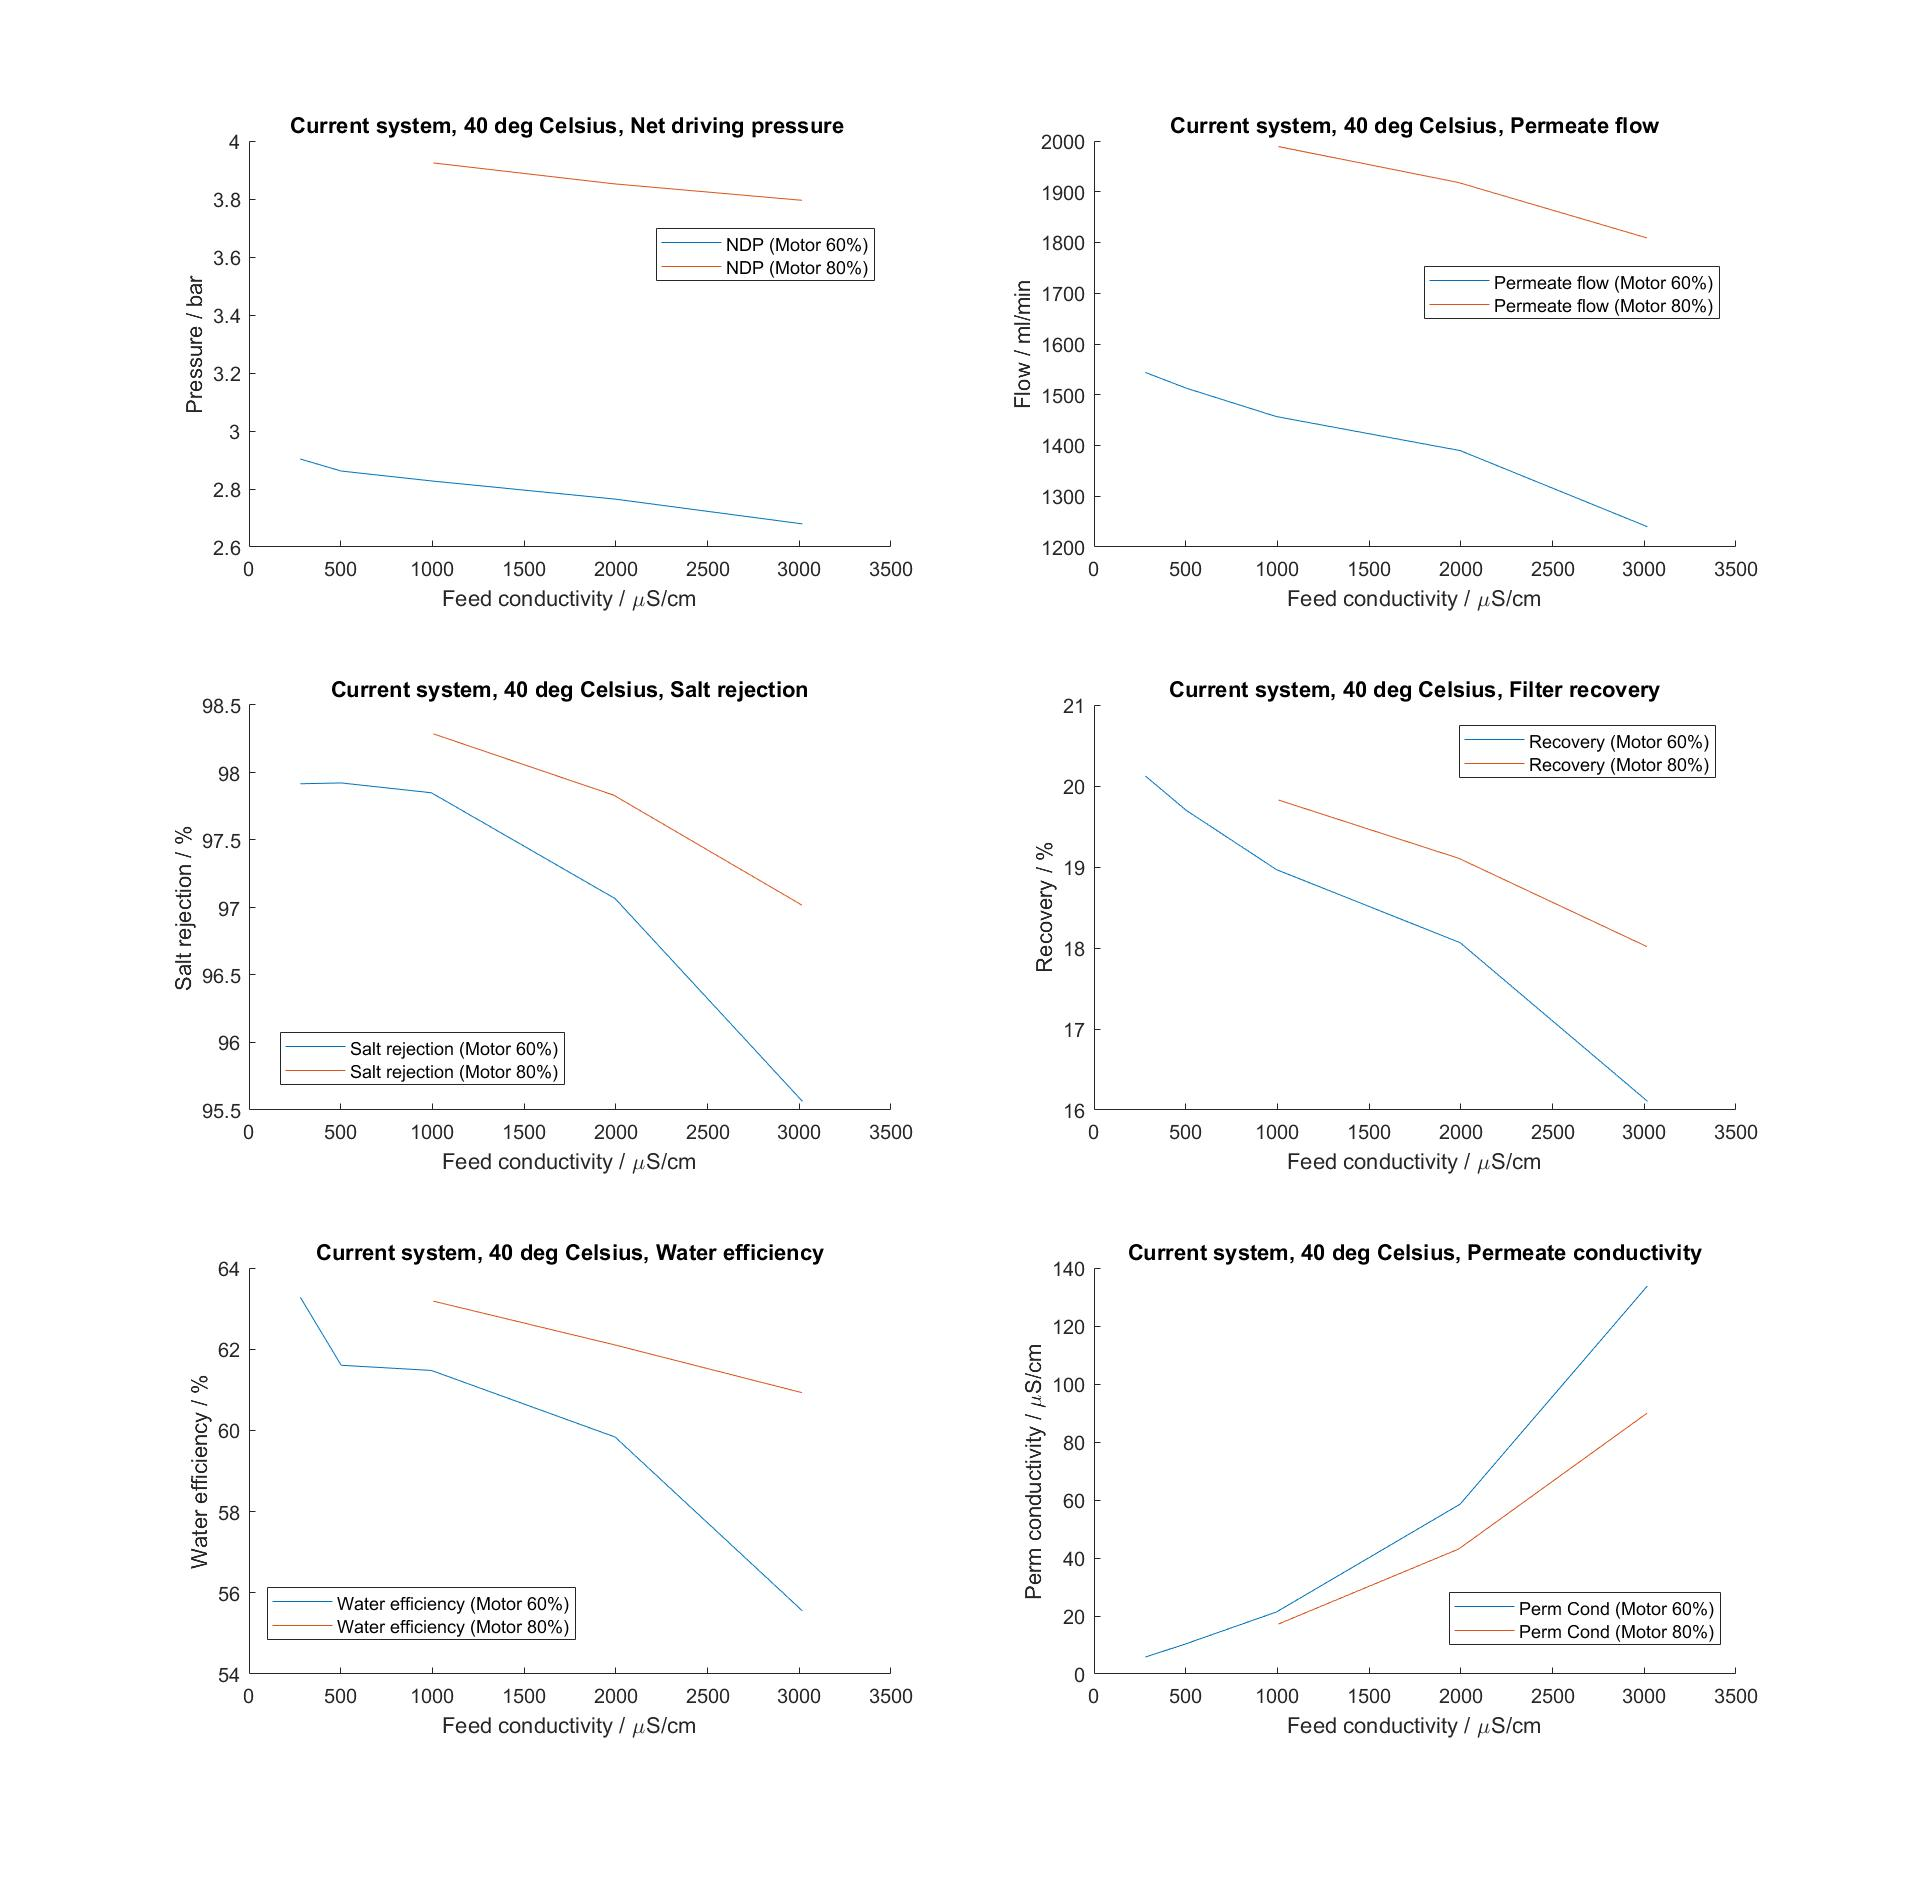
\includegraphics[width=1.1\textwidth]{Key40}
    \caption{Connections Pressure sensors}
    \label{fig:PressConn}
\end{figure}

\newpage

In order to understand how the system current performed in different working conditions all plots from the post processing in Matlab was put togheter. 

Net driving pressure was decreased when the temperature was increased. Higher feed conductivity resulted in a decreased net driving pressure. As expected, running the feed pump at a higher RPM also increased the net driving pressure.



\begin{figure}[H]
    \centering
    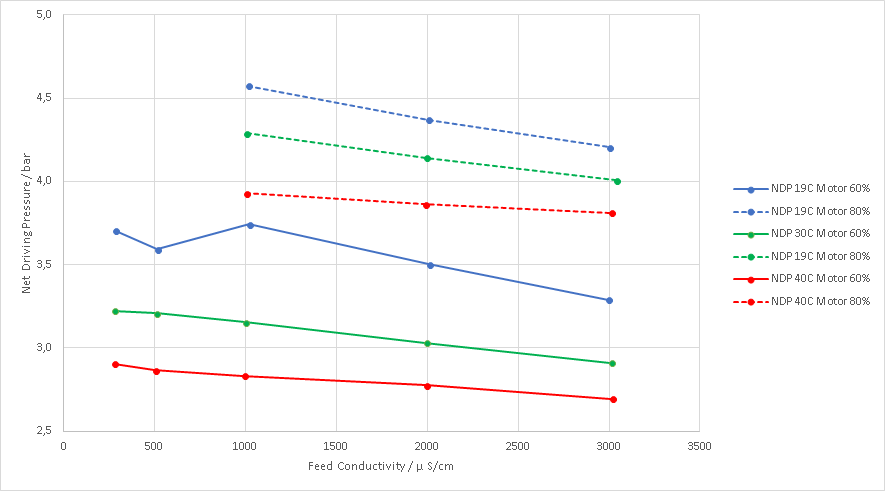
\includegraphics[width=1.1\textwidth]{NDP}
    \caption{Connections Pressure sensors}
    \label{fig:PressConn}
\end{figure}


\begin{figure}[H]
    \centering
    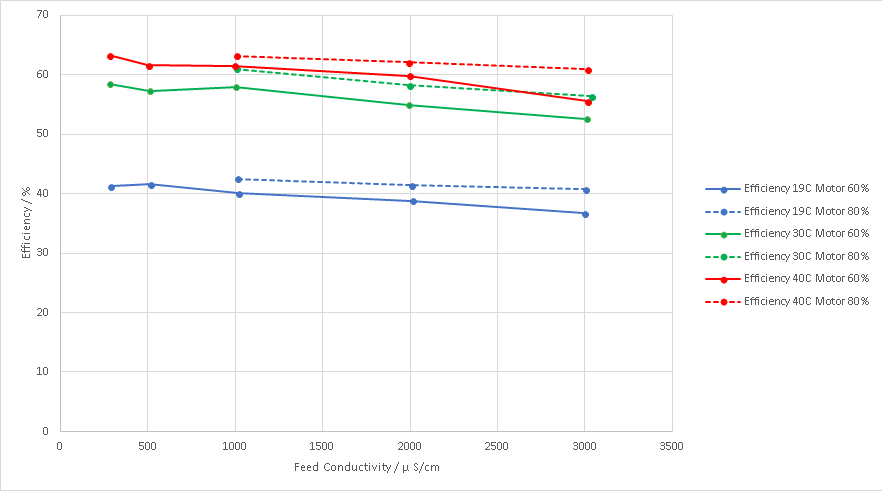
\includegraphics[width=1.1\textwidth]{Efficiency}
    \caption{Connections Pressure sensors}
    \label{fig:PressConn}
\end{figure}

\begin{figure}[H]
    \centering
    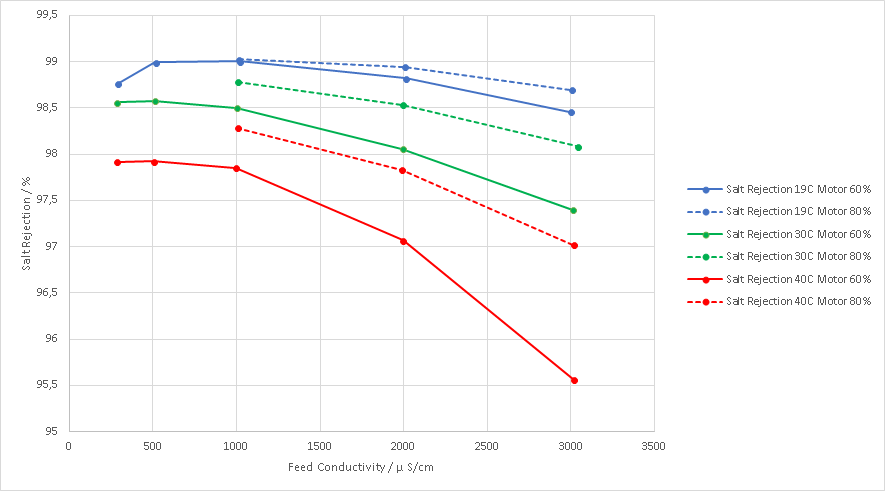
\includegraphics[width=1.1\textwidth]{SaltRejection}
    \caption{Connections Pressure sensors}
    \label{fig:PressConn}
\end{figure}

\begin{figure}[H]
    \centering
    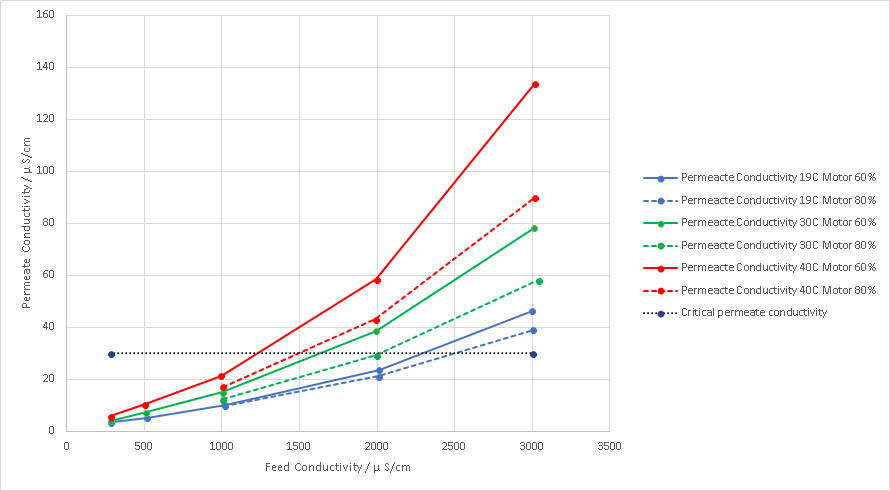
\includegraphics[width=1.1\textwidth]{PermCond}
    \caption{Connections Pressure sensors}
    \label{fig:PressConn}
\end{figure}

Summary results recovery:

Warmer water enabled more feed water to pass through the membrane and therefore the recovery was increased. Increased conductivity reduced recovery due to the increased net driving pressure. 

\begin{figure}[H]
    \centering
    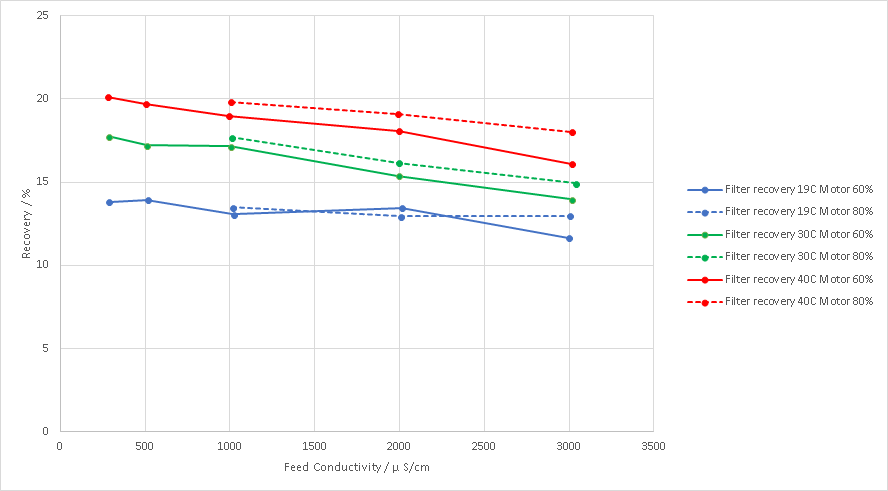
\includegraphics[width=1.1\textwidth]{Recovery}
    \caption{Connections Pressure sensors}
    \label{fig:PressConn}
\end{figure}


\begin{figure}[H]
    \centering
    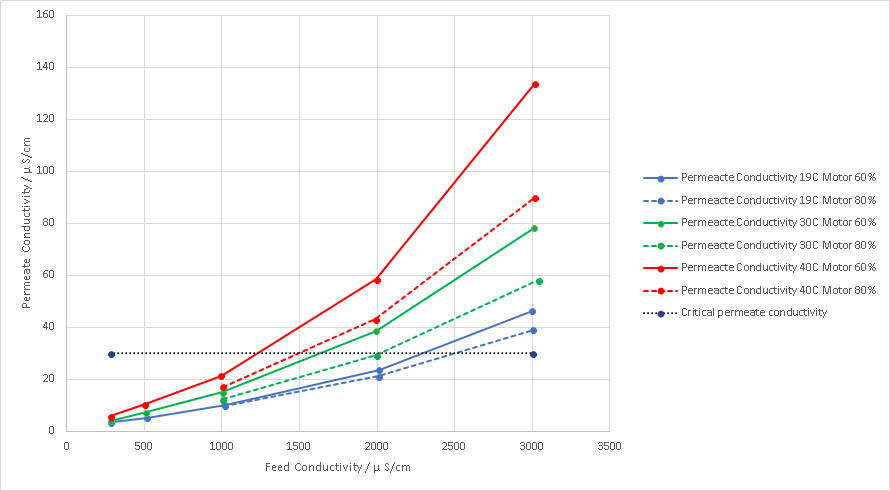
\includegraphics[width=1.1\textwidth]{PermCond}
    \caption{Connections Pressure sensors}
    \label{fig:PressConn}
\end{figure}





\subsection{System 2}

Test: increased feed pressure

21


\begin{figure}[H]
    \centering
    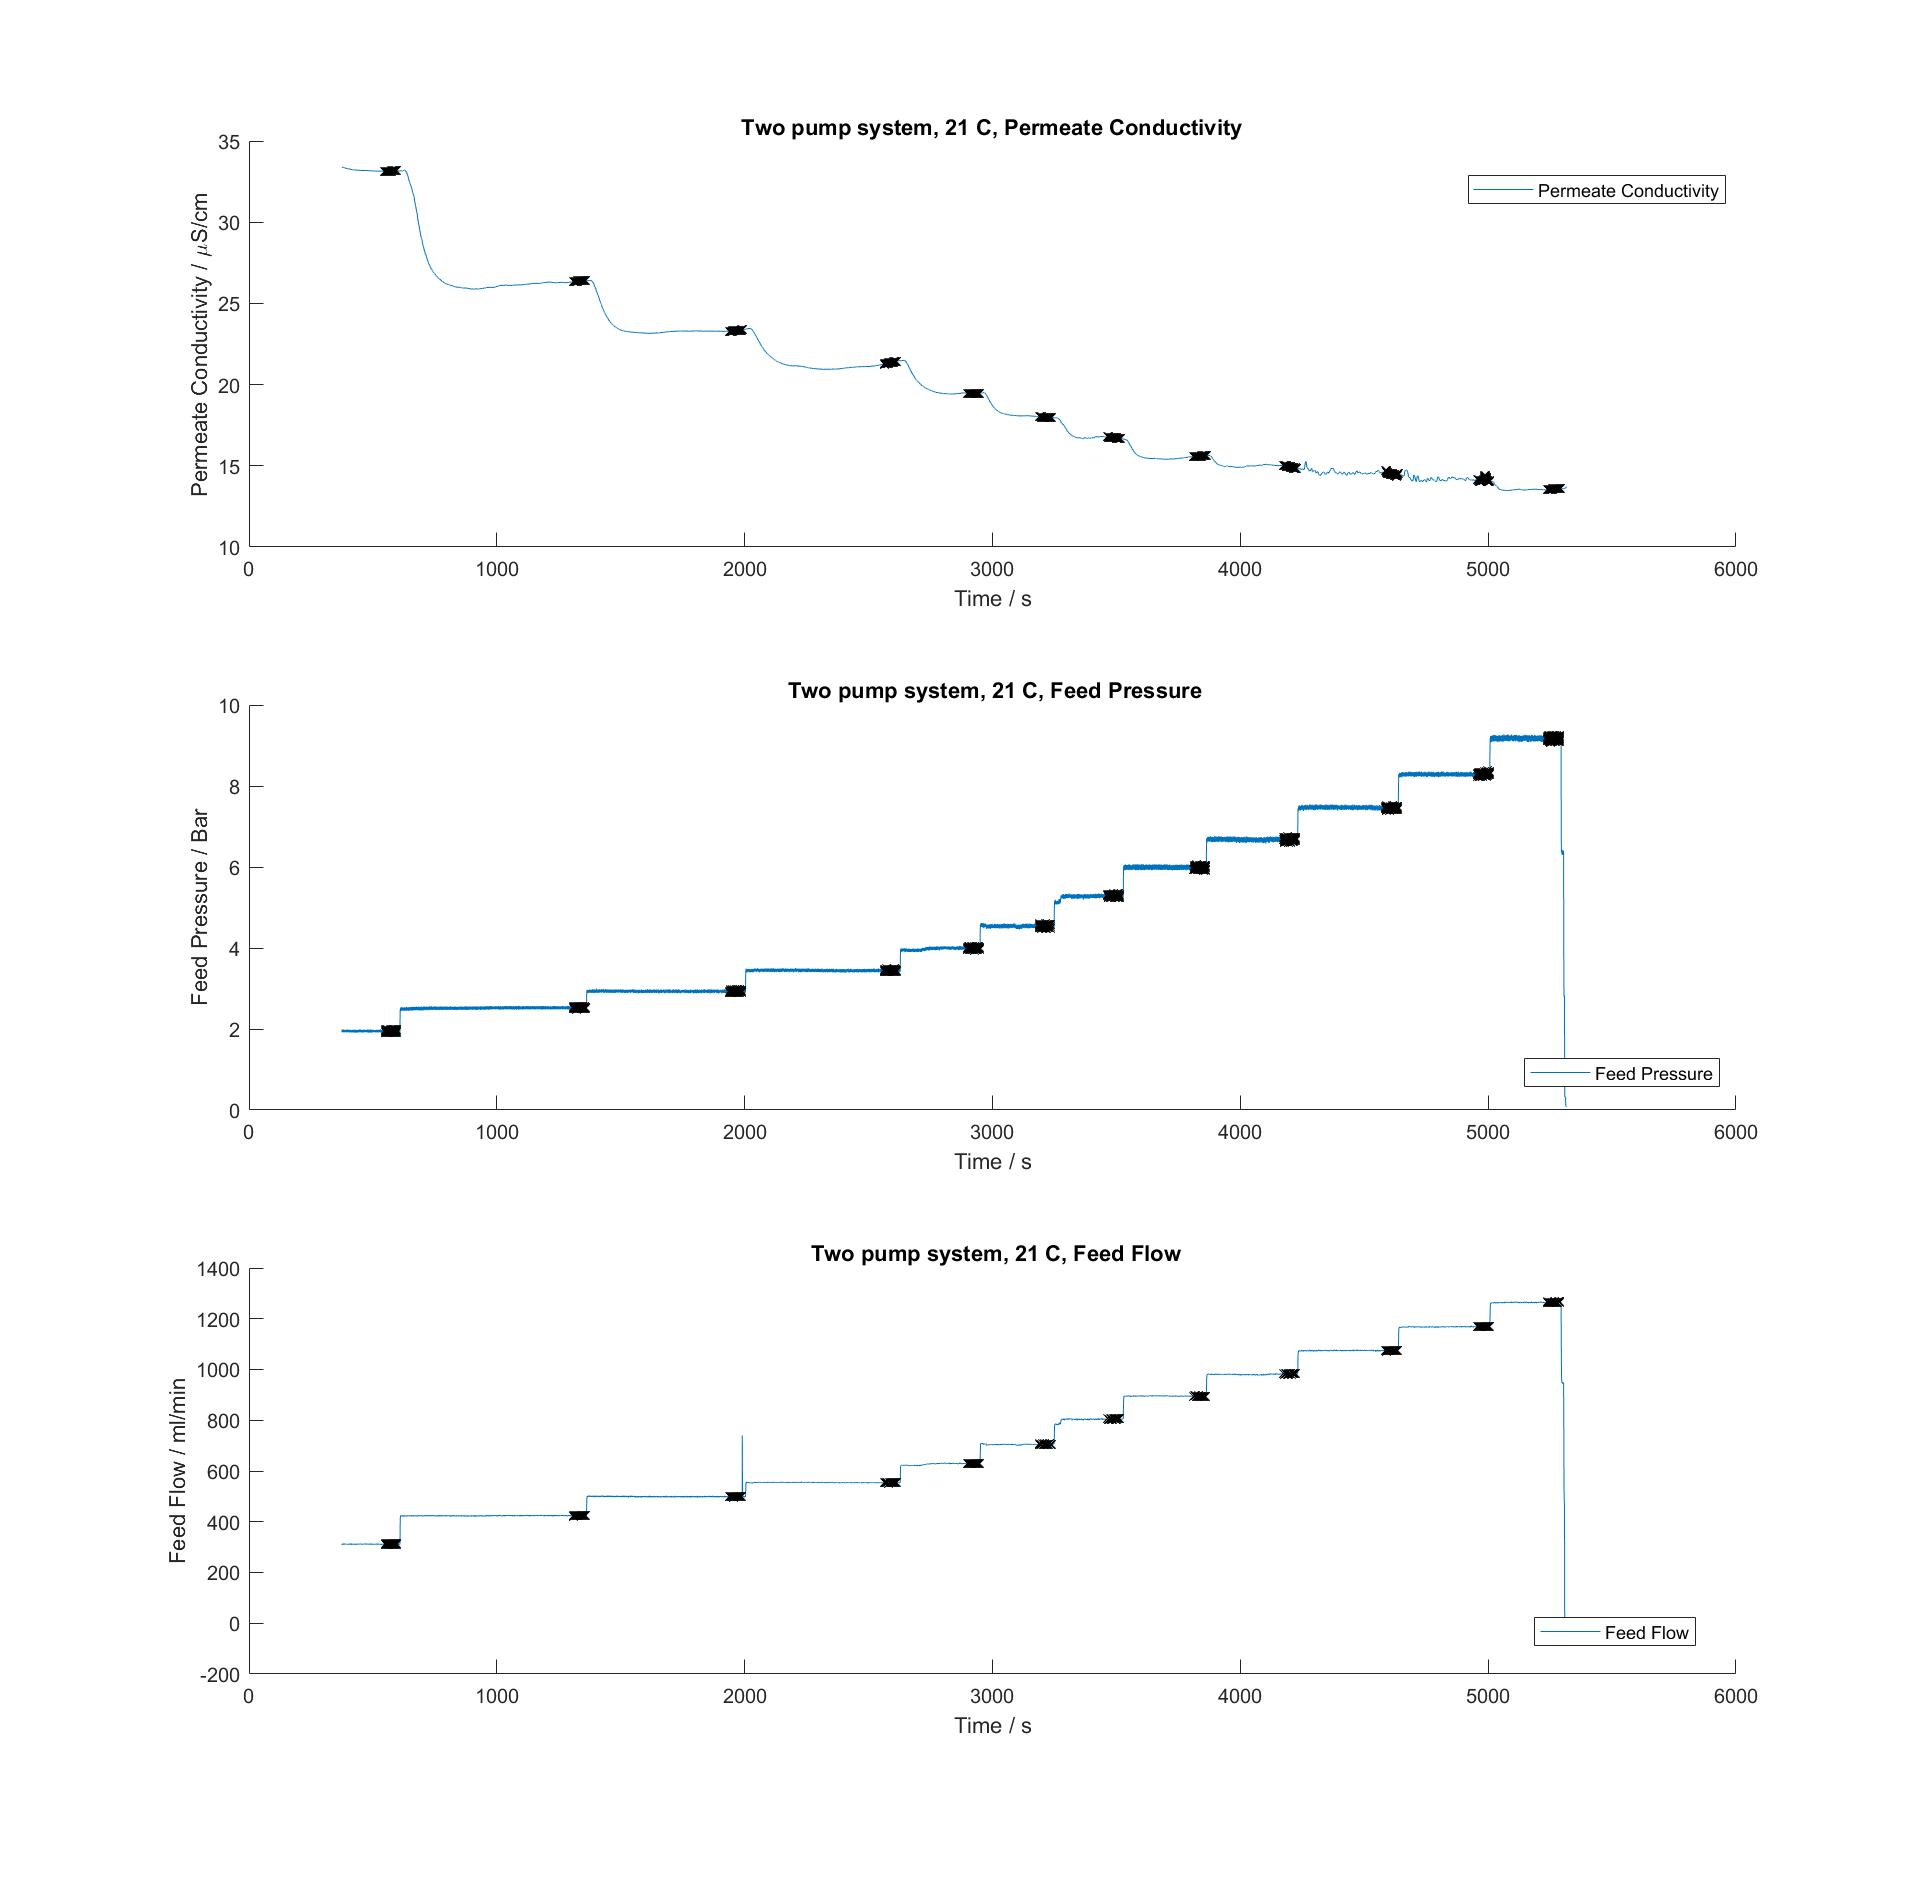
\includegraphics[width=1.1\textwidth]{FeedPumpIncrease21}
    \caption{Connections Pressure sensors}
    \label{fig:PressConn}
\end{figure}


\begin{figure}[H]
    \centering
    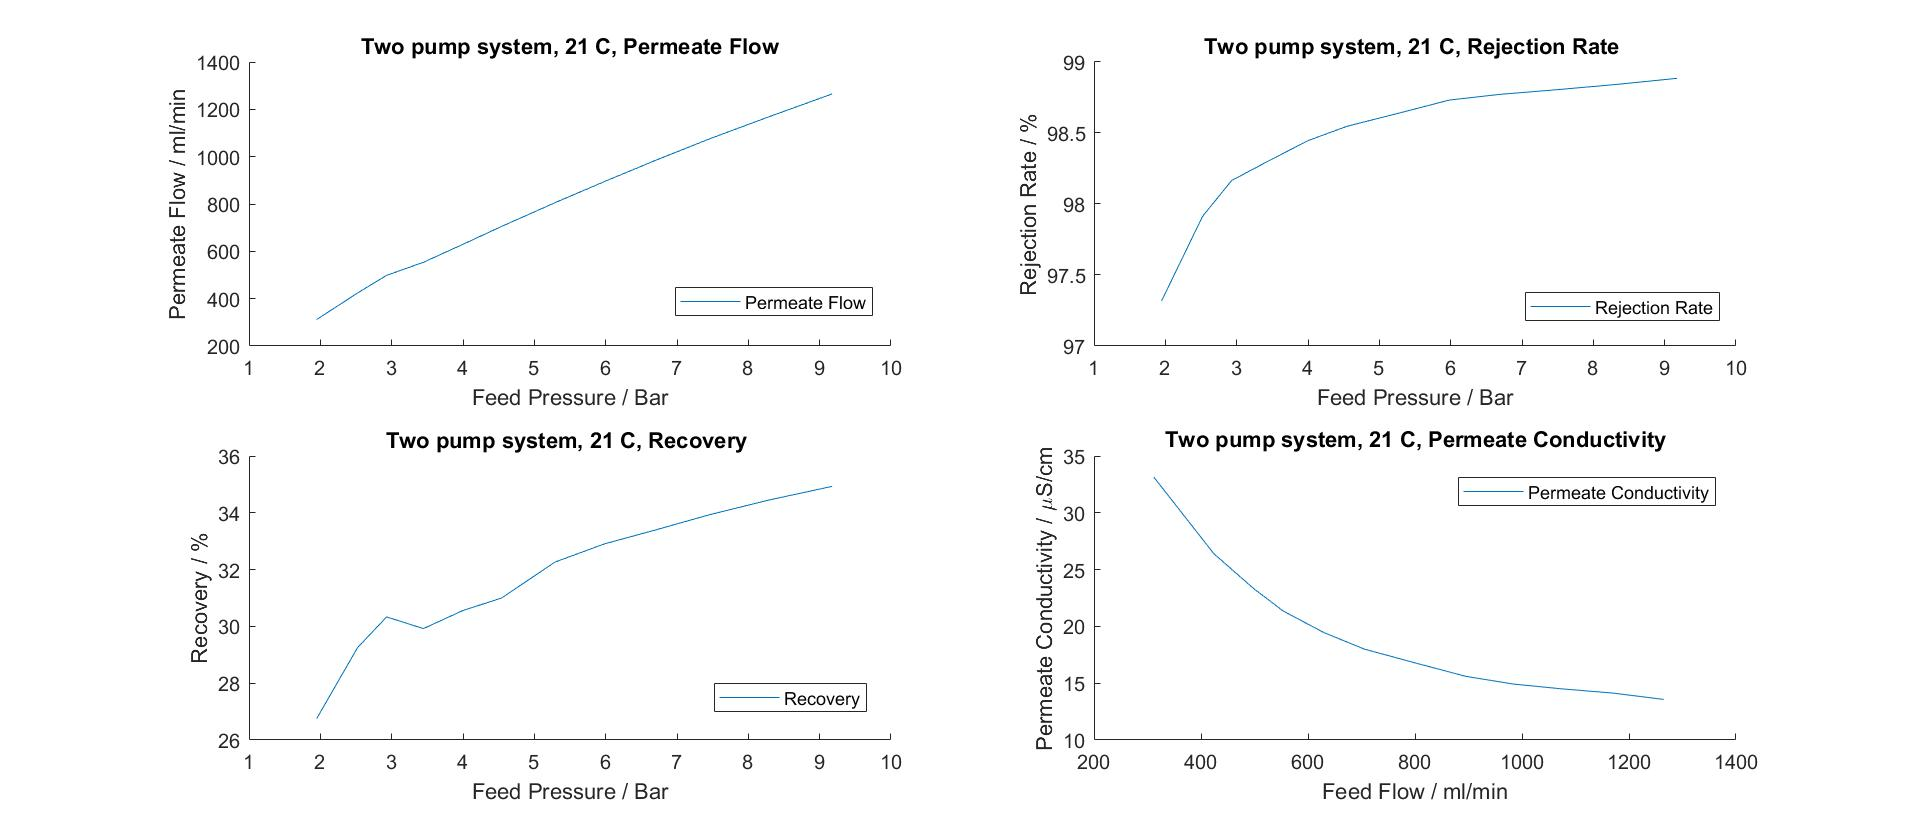
\includegraphics[width=1.1\textwidth]{FeedPumpIncrease21Key}
    \caption{Connections Pressure sensors}
    \label{fig:PressConn}
\end{figure}

30


\begin{figure}[H]
    \centering
    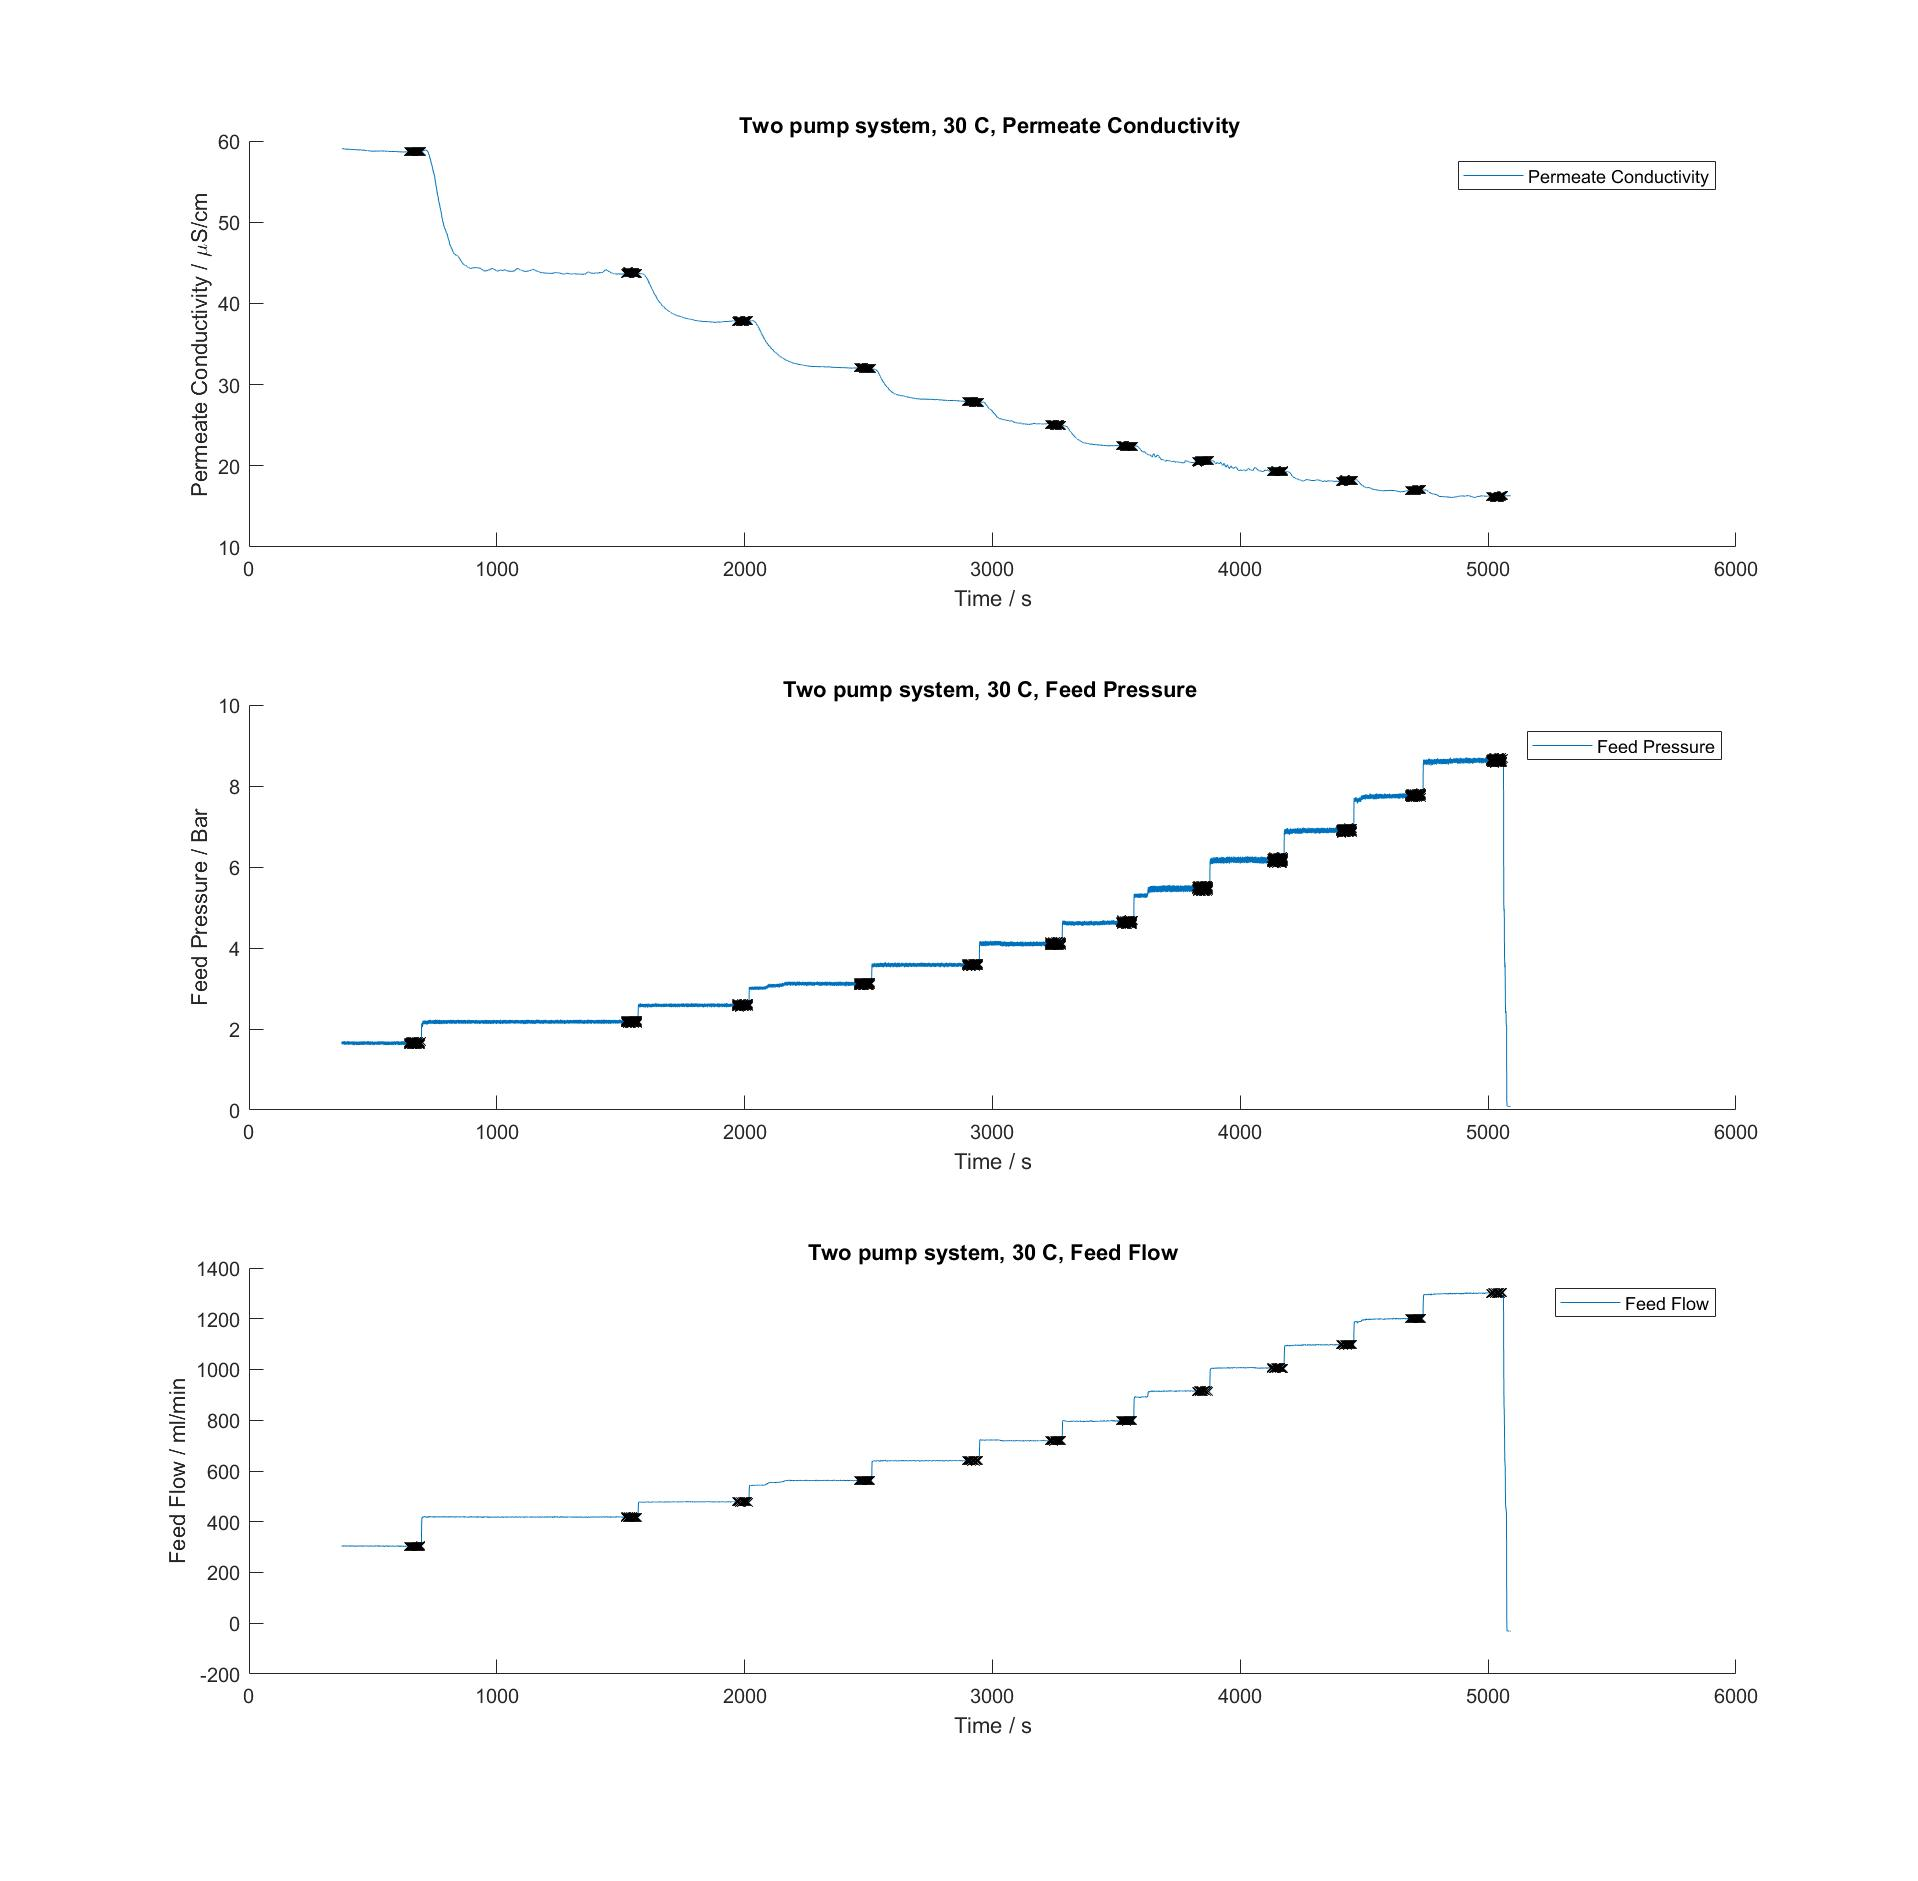
\includegraphics[width=1.1\textwidth]{FeedPumpIncrease30}
    \caption{Connections Pressure sensors}
    \label{fig:PressConn}
\end{figure}


\begin{figure}[H]
    \centering
    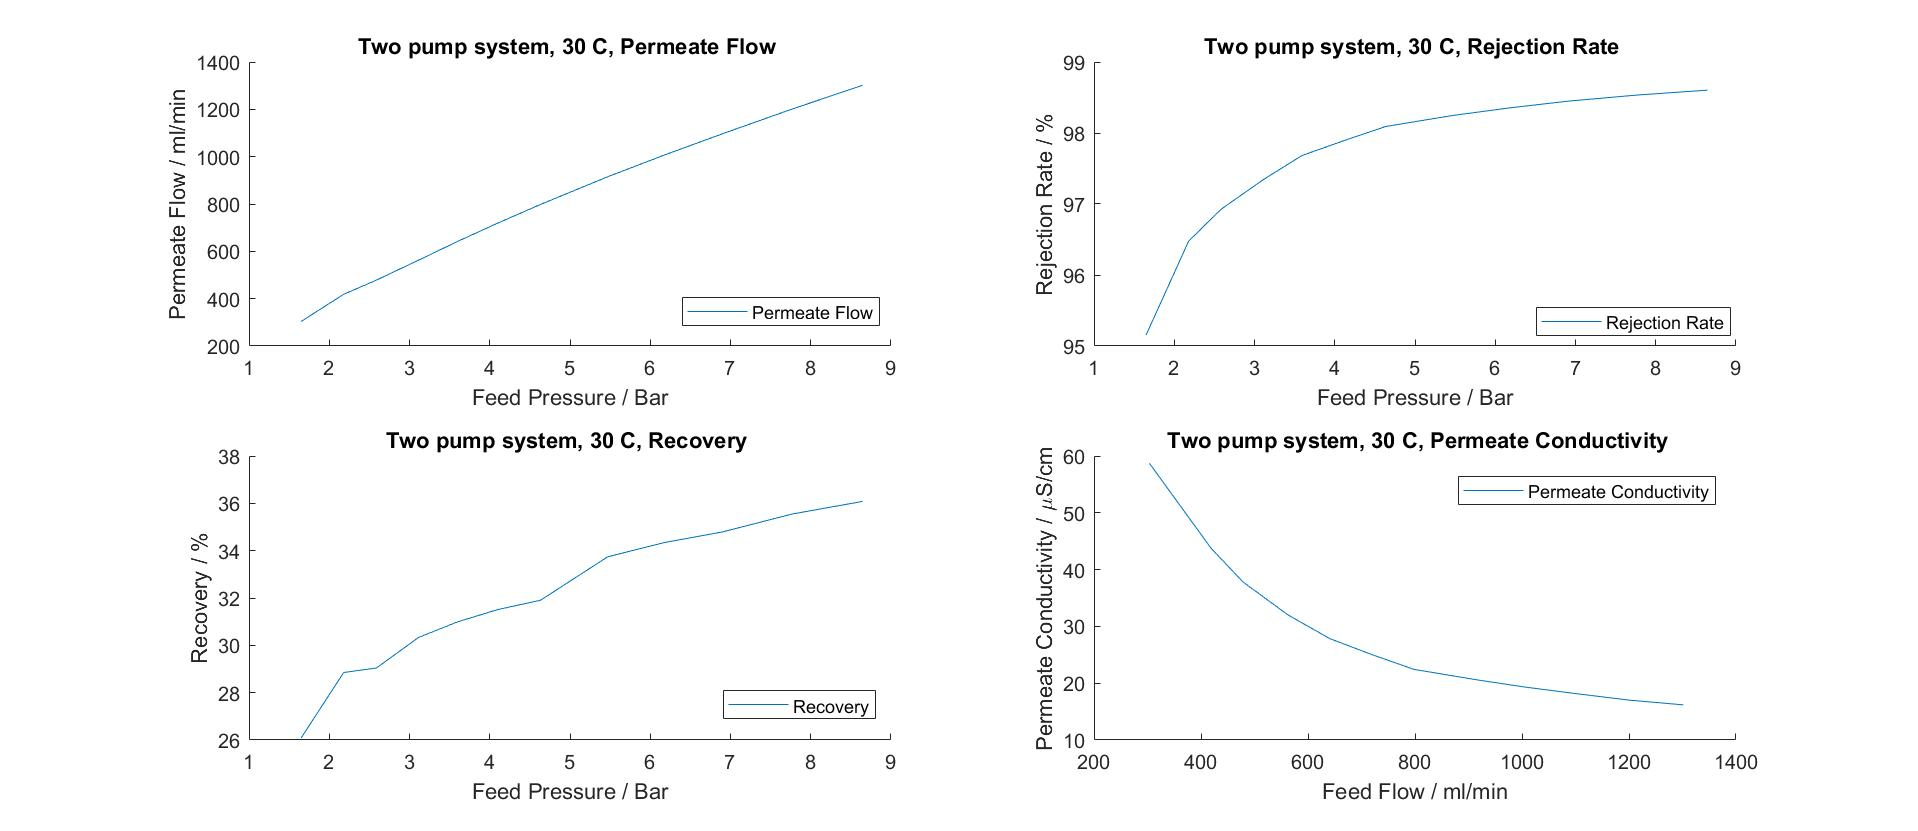
\includegraphics[width=1.1\textwidth]{FeedPumpIncrease30Key}
    \caption{Connections Pressure sensors}
    \label{fig:PressConn}
\end{figure}

40


\begin{figure}[H]
    \centering
    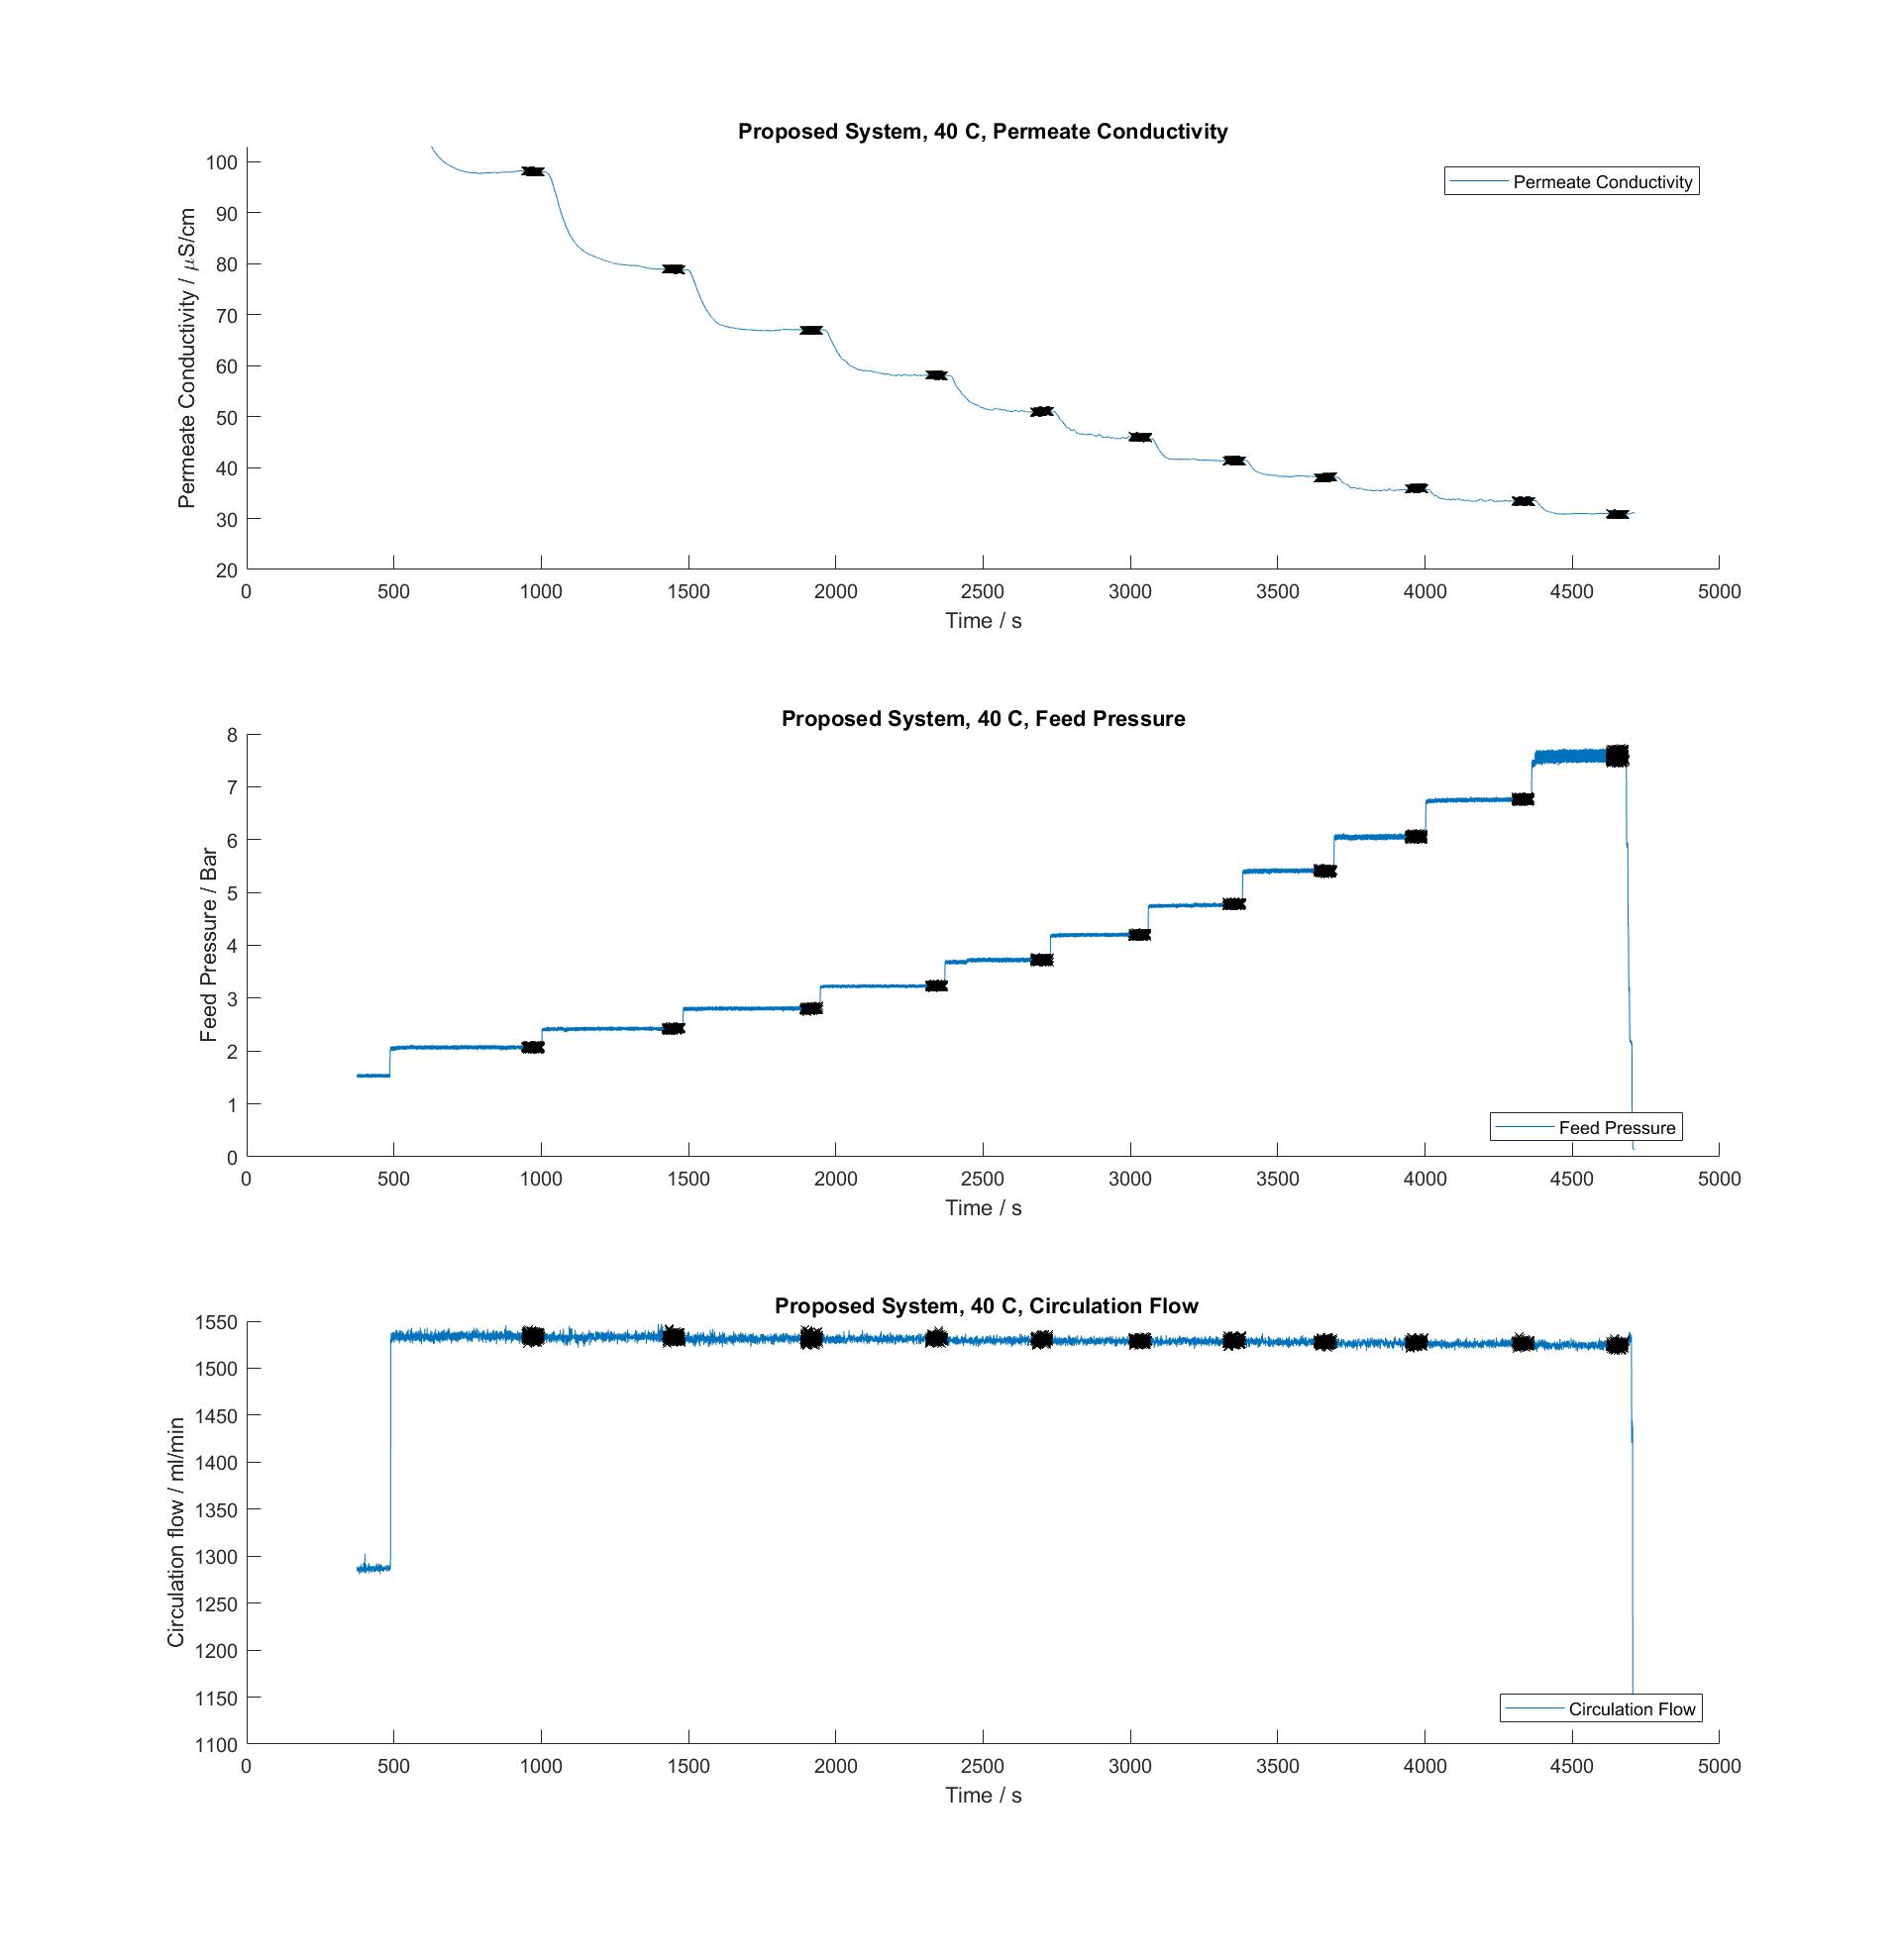
\includegraphics[width=1.1\textwidth]{FeedPumpIncrease40}
    \caption{Connections Pressure sensors}
    \label{fig:PressConn}
\end{figure}


\begin{figure}[H]
    \centering
    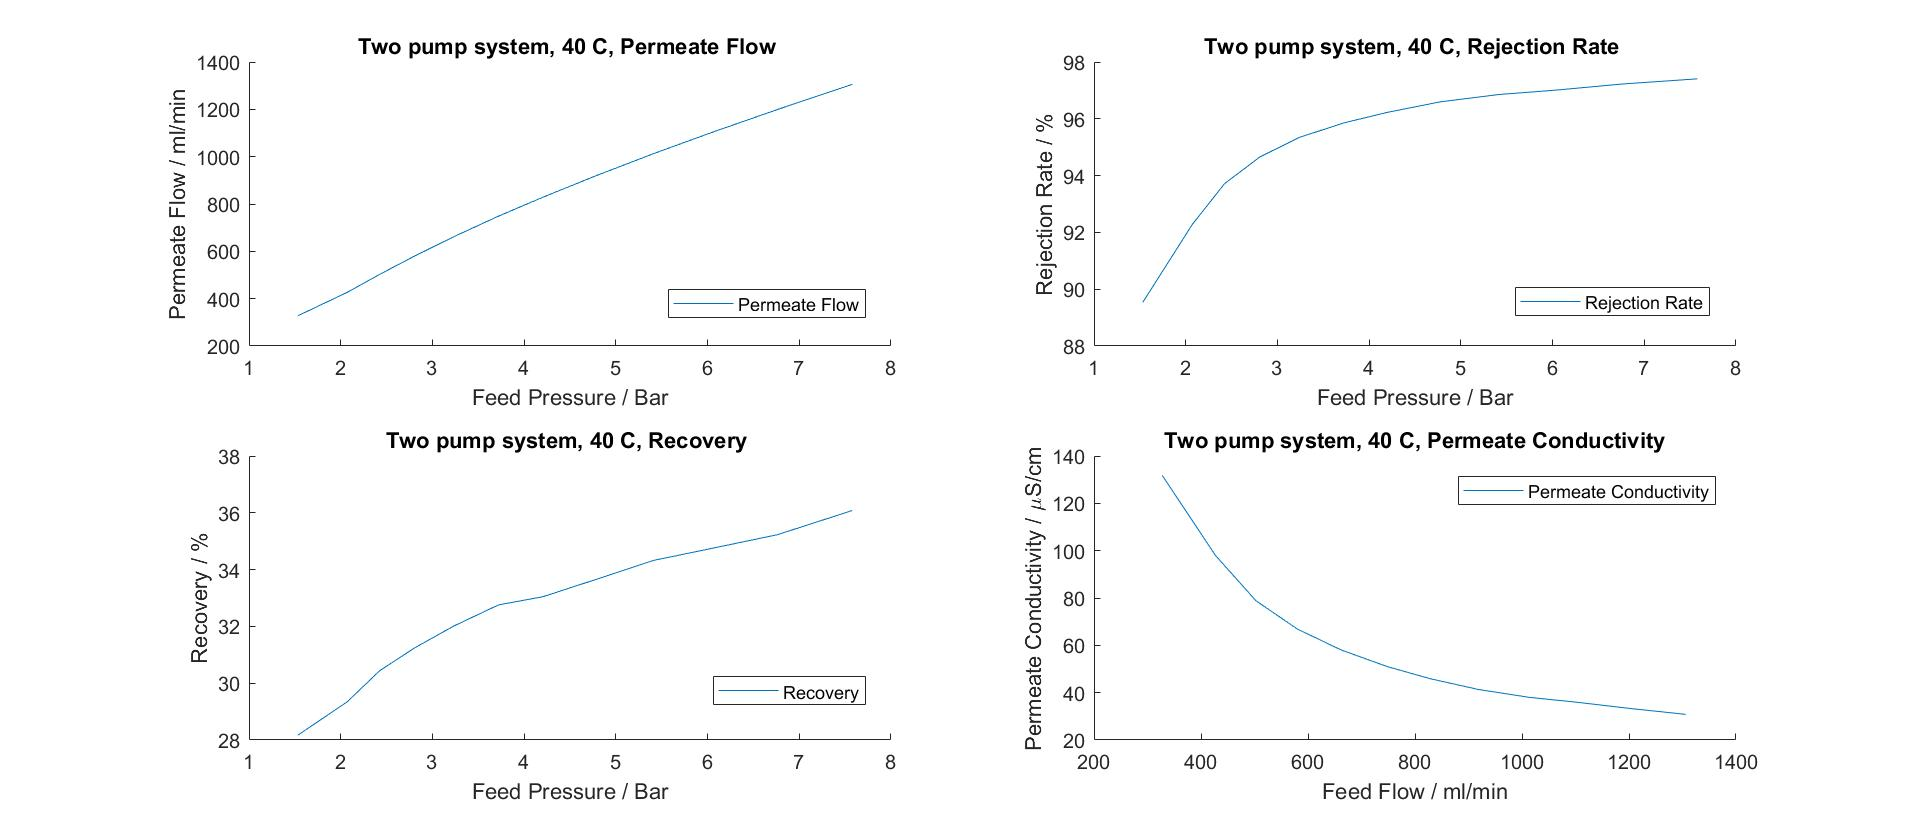
\includegraphics[width=1.1\textwidth]{FeedPumpIncrease40Key}
    \caption{Connections Pressure sensors}
    \label{fig:PressConn}
\end{figure}

Recovery Increase

\begin{figure}[H]
    \centering
    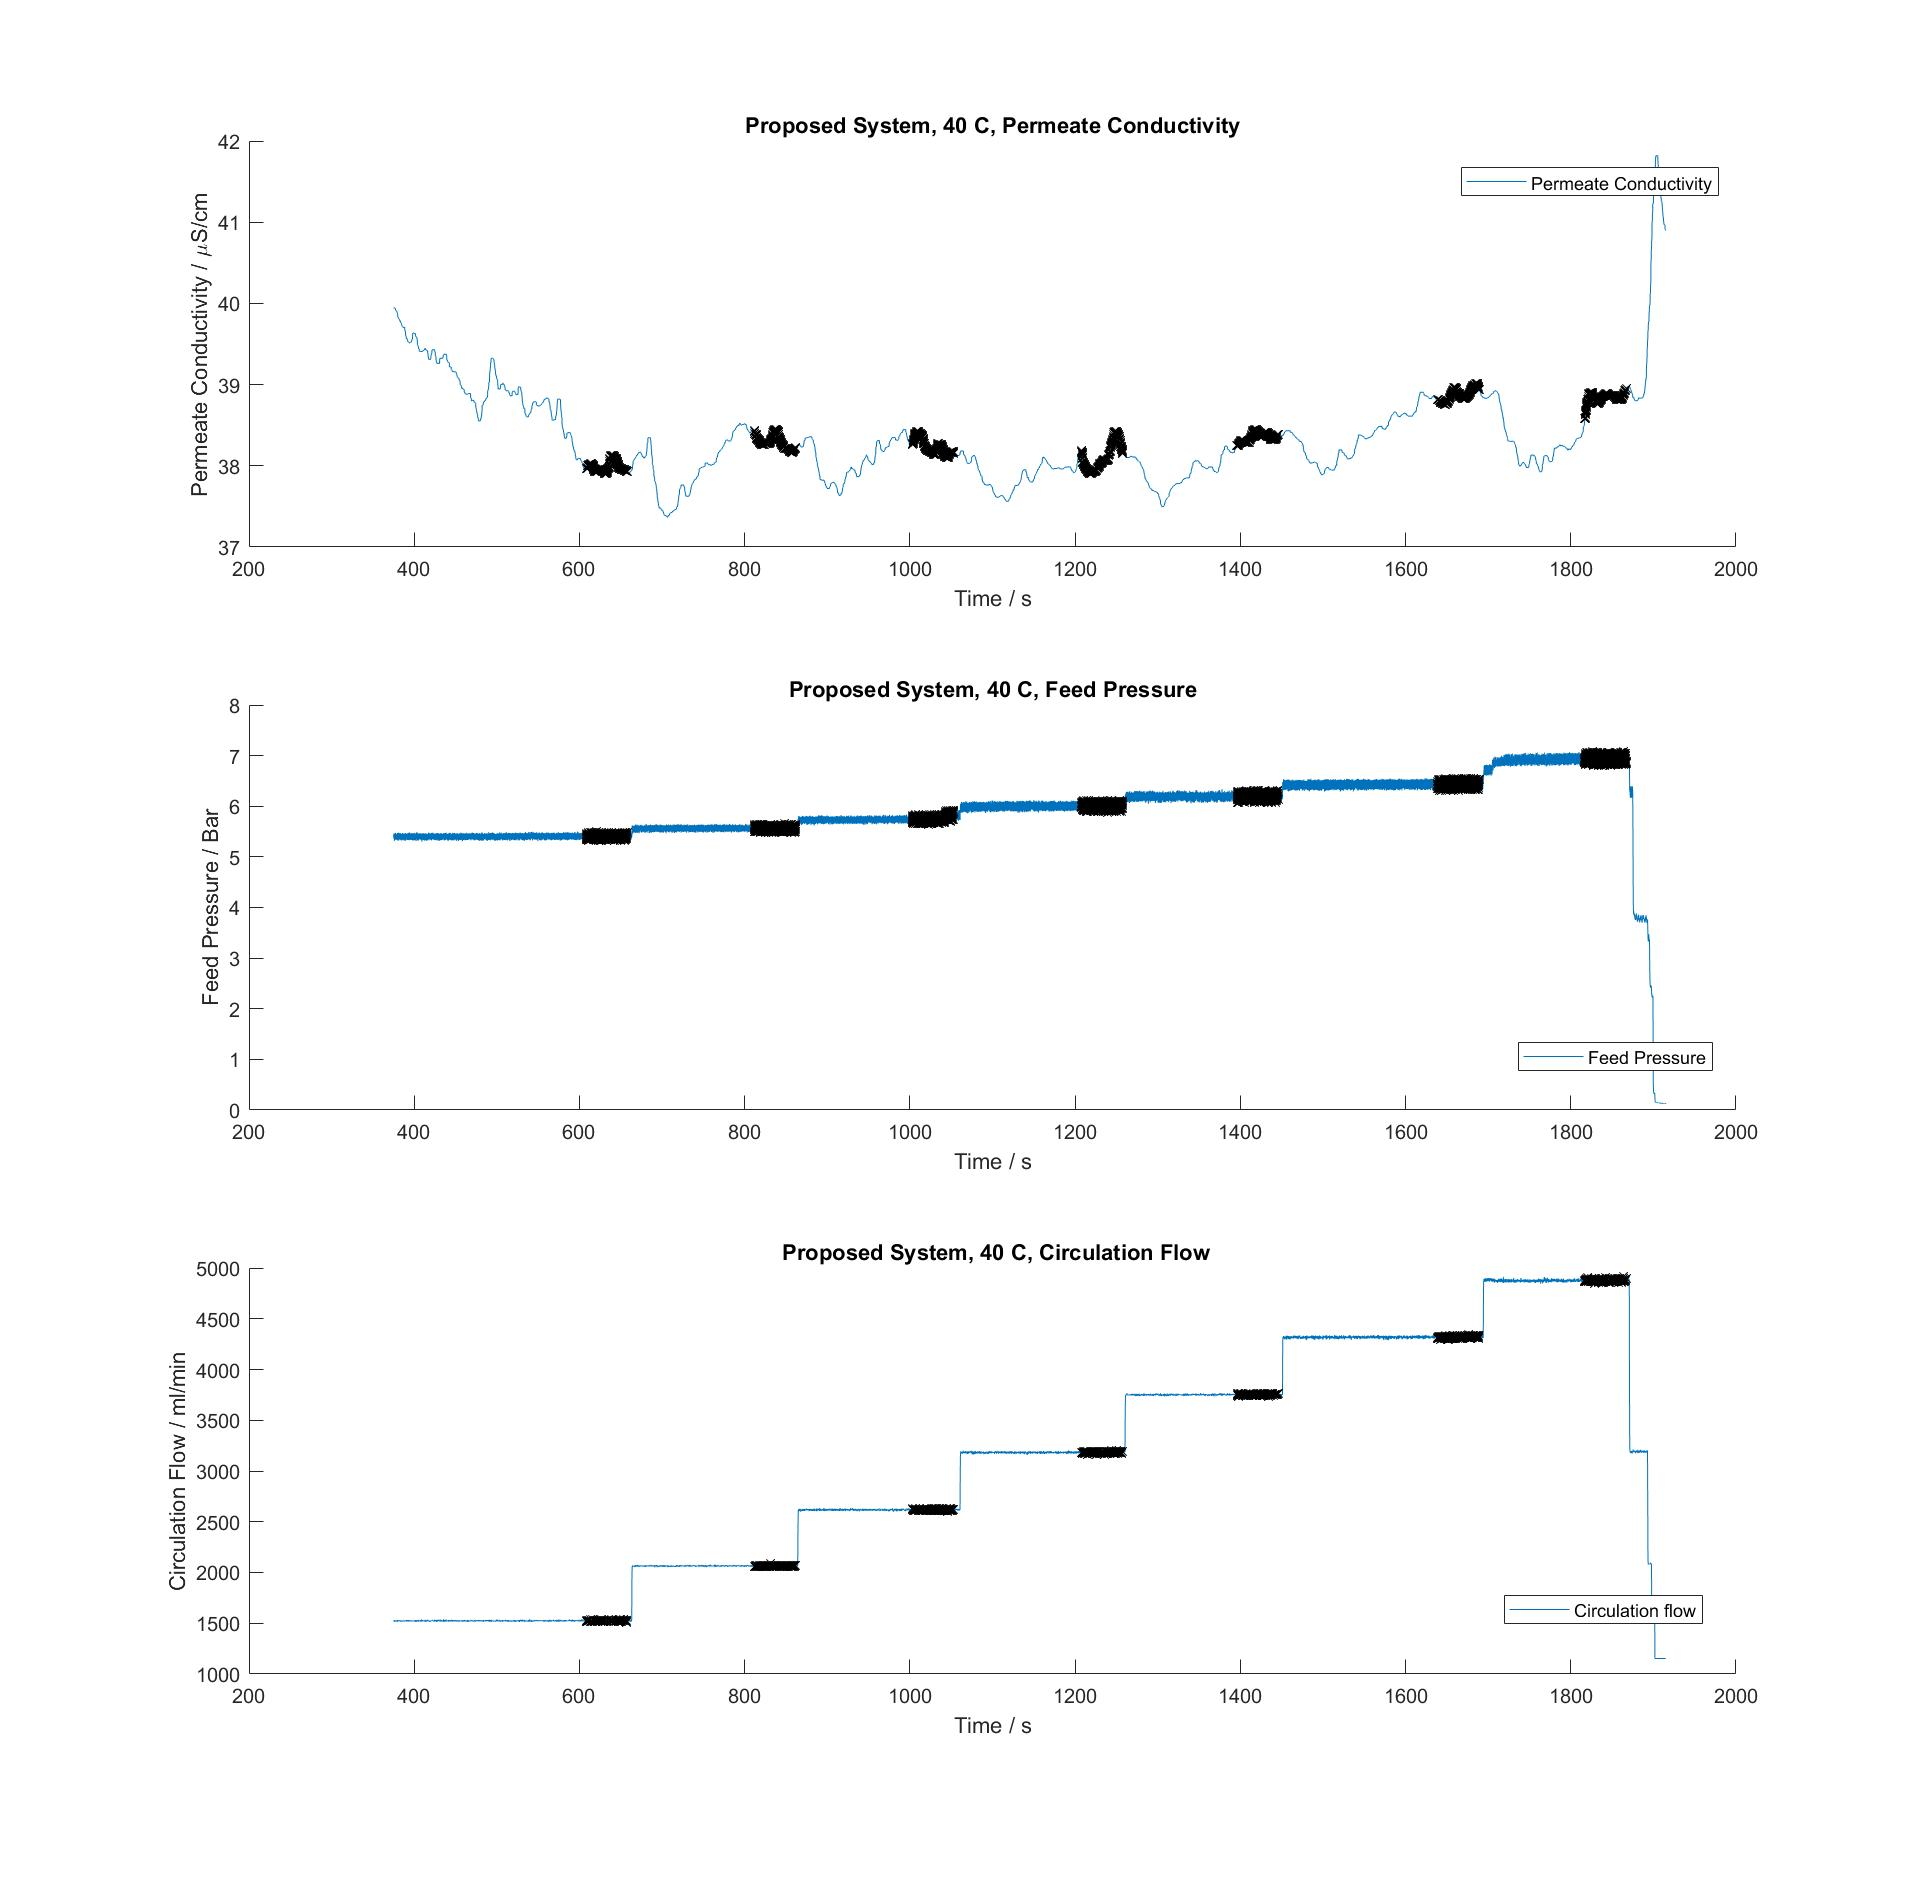
\includegraphics[width=1.1\textwidth]{RecIncrease40}
    \caption{Connections Pressure sensors}
    \label{fig:PressConn}
\end{figure}

\begin{figure}[H]
    \centering
    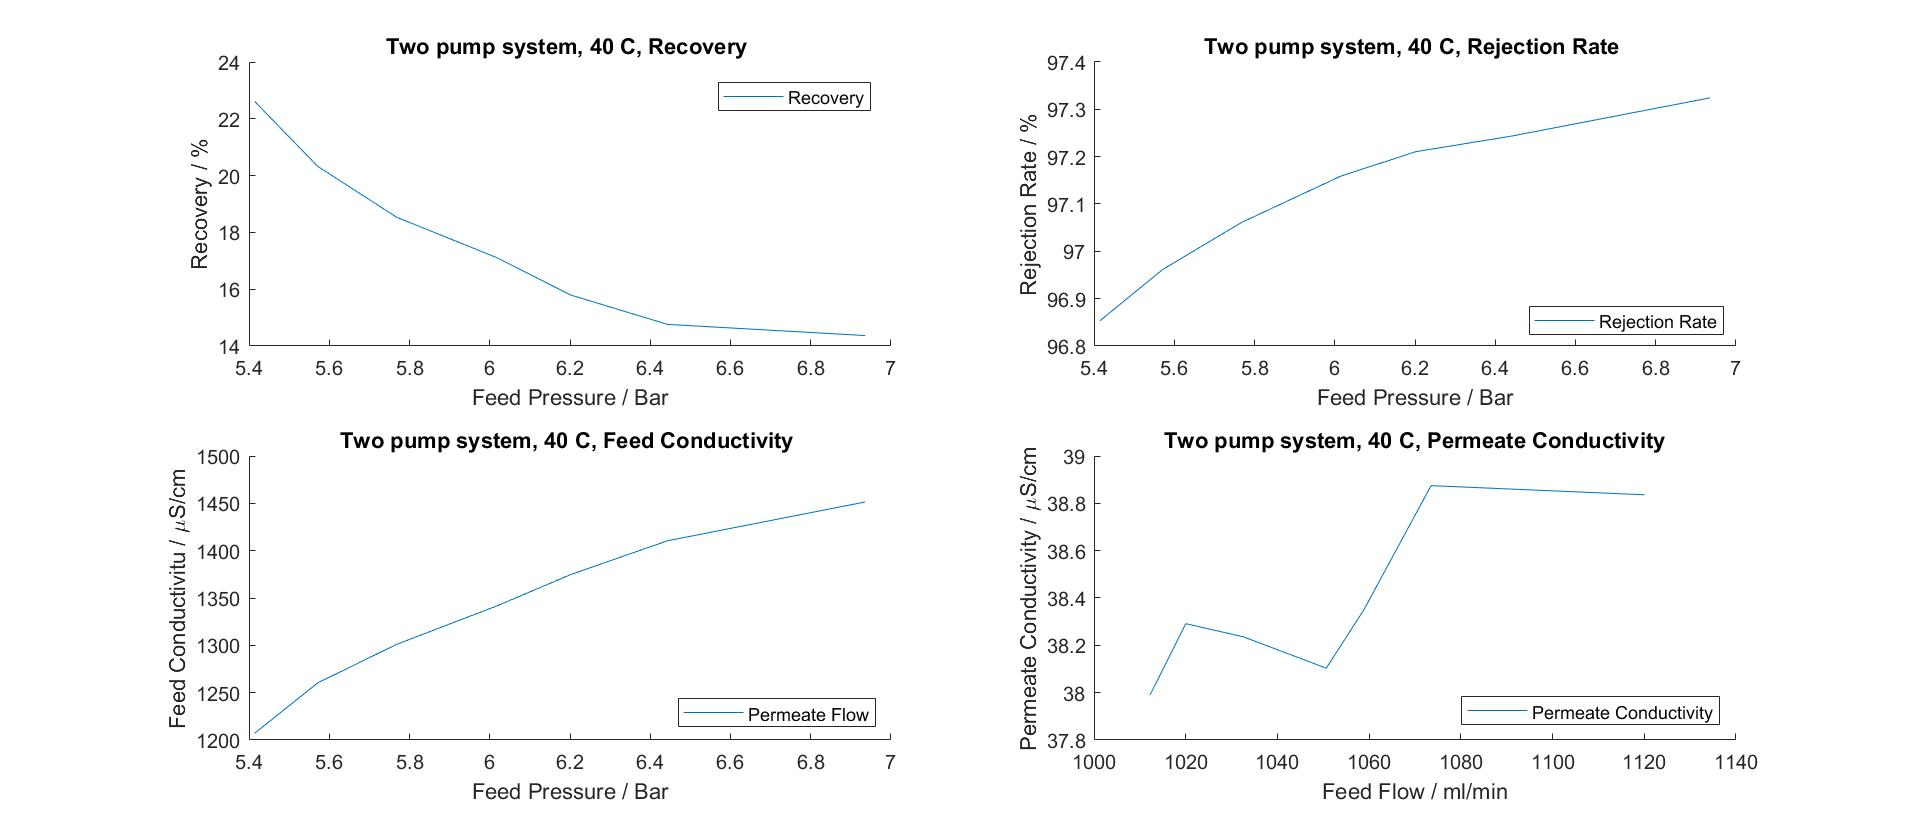
\includegraphics[width=1.1\textwidth]{RecIncrease40Key}
    \caption{Connections Pressure sensors}
    \label{fig:PressConn}
\end{figure}



\section{Implementation Test Rig}


\subsection{Connections}
In Figure (\ref{fig:PressConn}-\ref{fig:PumpConn}) all connections in the test rig is displayed.


\begin{figure}[h]
    \centering
    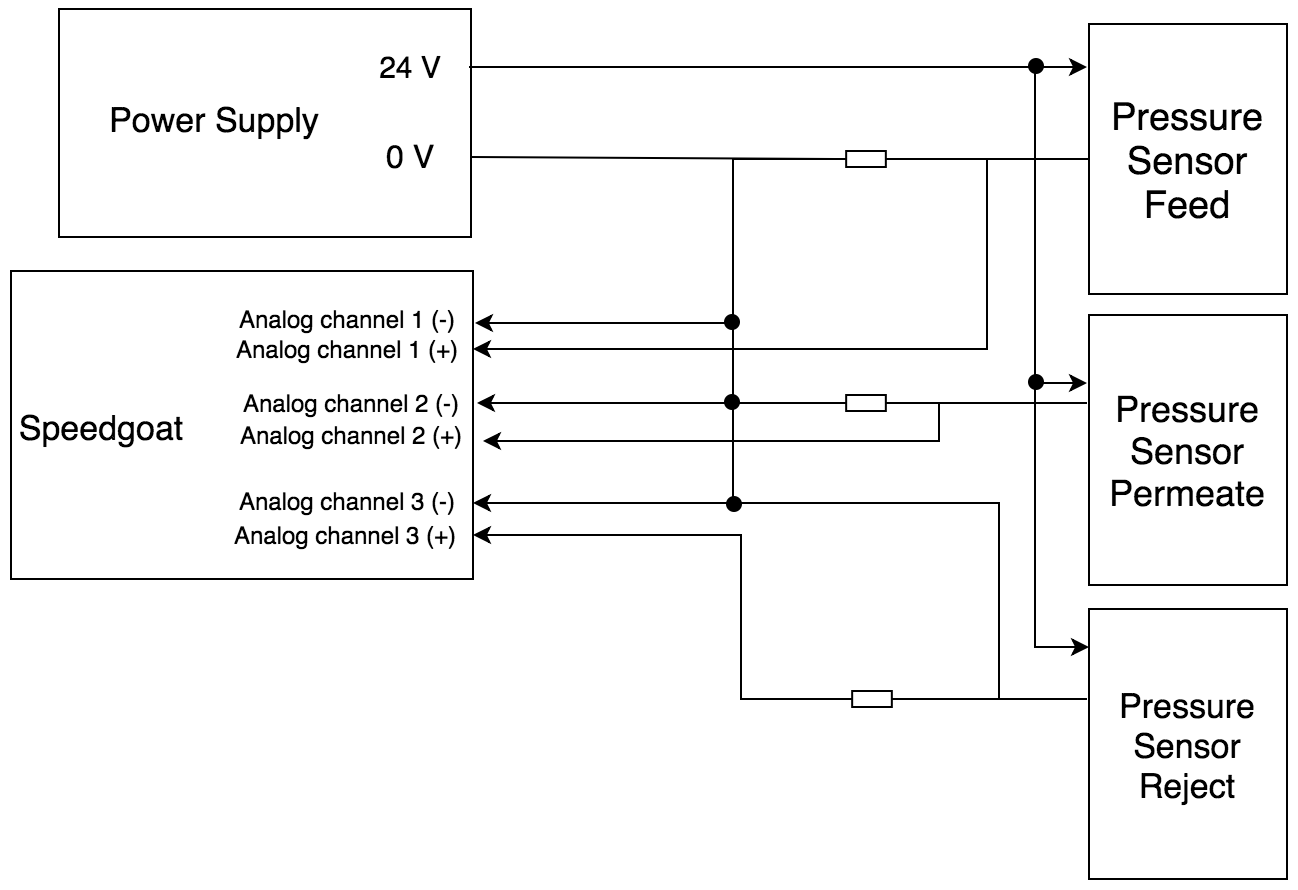
\includegraphics[width=0.7\textwidth]{PressConn}
    \caption{Connections Pressure sensors}
    \label{fig:PressConn}
\end{figure}

\begin{figure}[h]
    \centering
    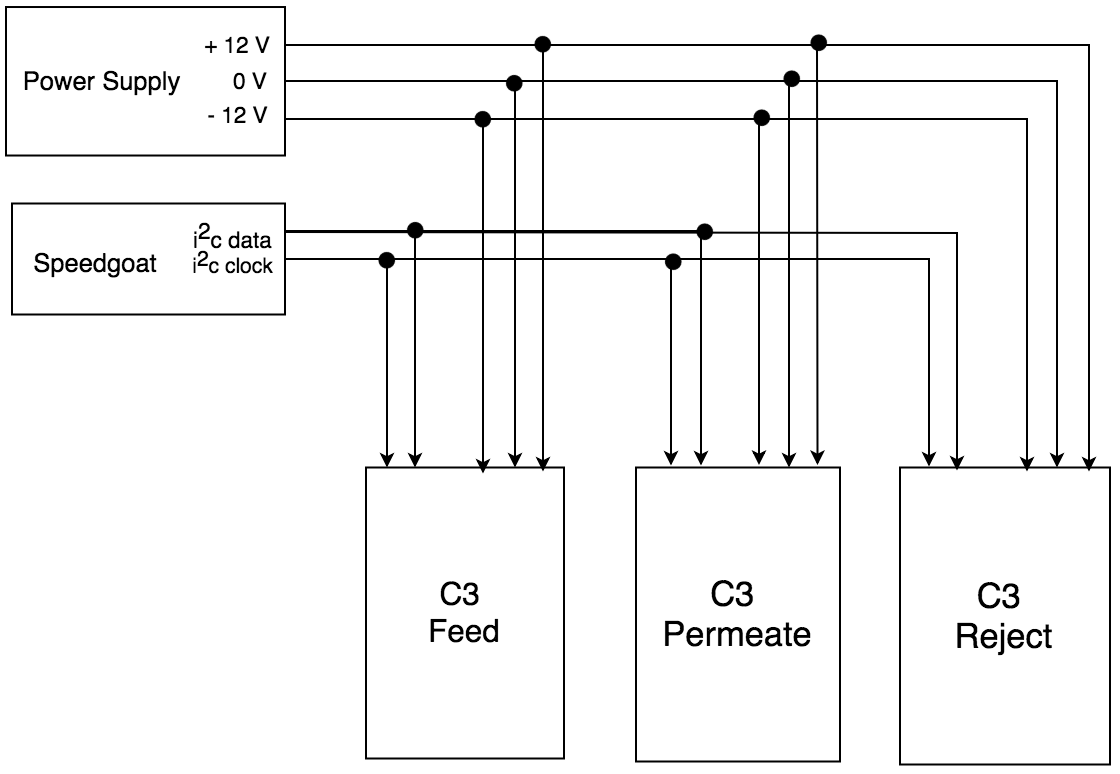
\includegraphics[width=0.7\textwidth]{C3Conn}
    \caption{Connections measurement blocks, C3}
    \label{fig:C3Conn}
\end{figure}

\begin{figure}[h]
    \centering
    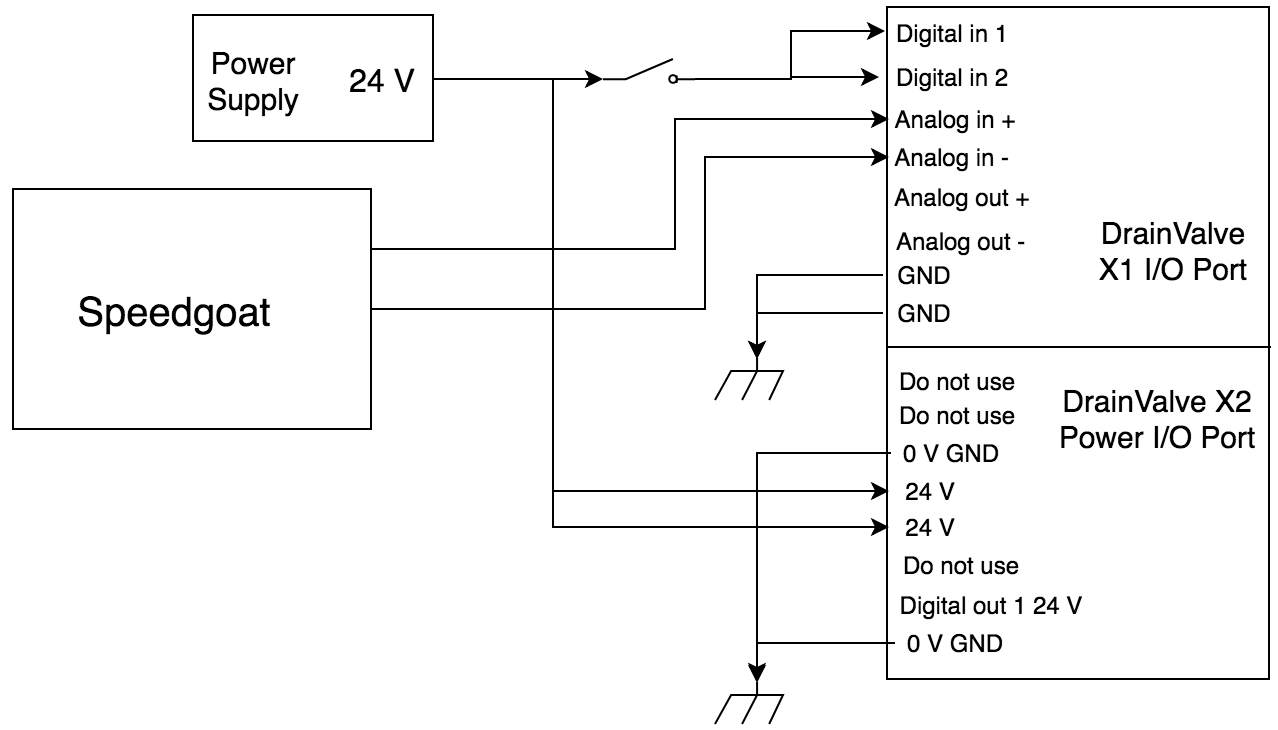
\includegraphics[width=0.7\textwidth]{ValveConn}
    \caption{Connections Drain Valve}
    \label{fig:ValveConn}
\end{figure}

\begin{figure}[h]
    \centering
    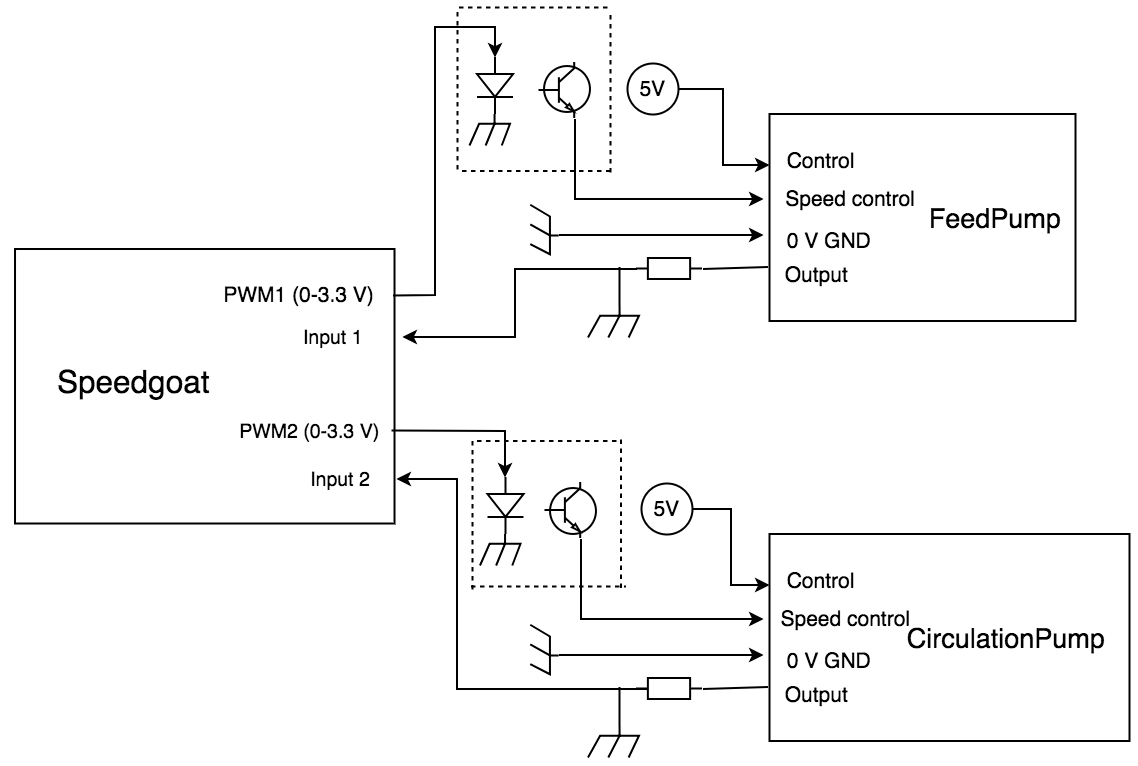
\includegraphics[width=0.7\textwidth]{PumpConn}
    \caption{Connections pumps}
    \label{fig:PumpConn}
\end{figure}


\section{Mapping}
\begin{figure}[h]
    \centering
    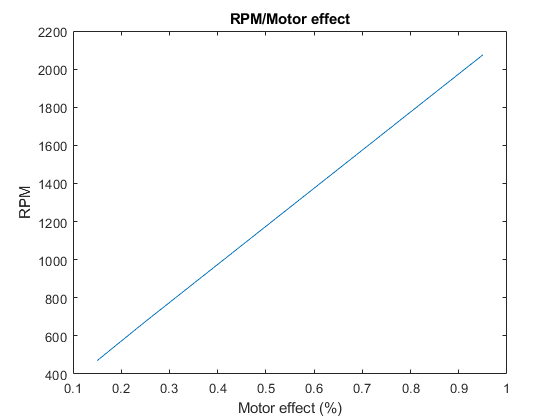
\includegraphics[width=0.7\textwidth]{RPM.png}
    \caption{RPM Pumps}
    \label{fig:RPM}
\end{figure}


\begin{figure}[h]
    \centering
    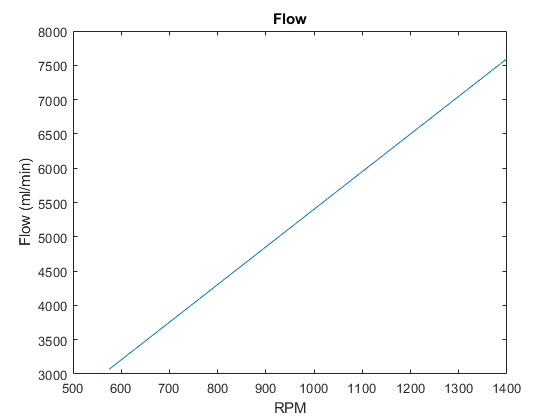
\includegraphics[width=0.7\textwidth]{Flow.png}
    \caption{Flowrate}
    \label{fig:Flowrate}
\end{figure}


\section{Design of control algorithms}

\begin{figure}[h]
    \centering
    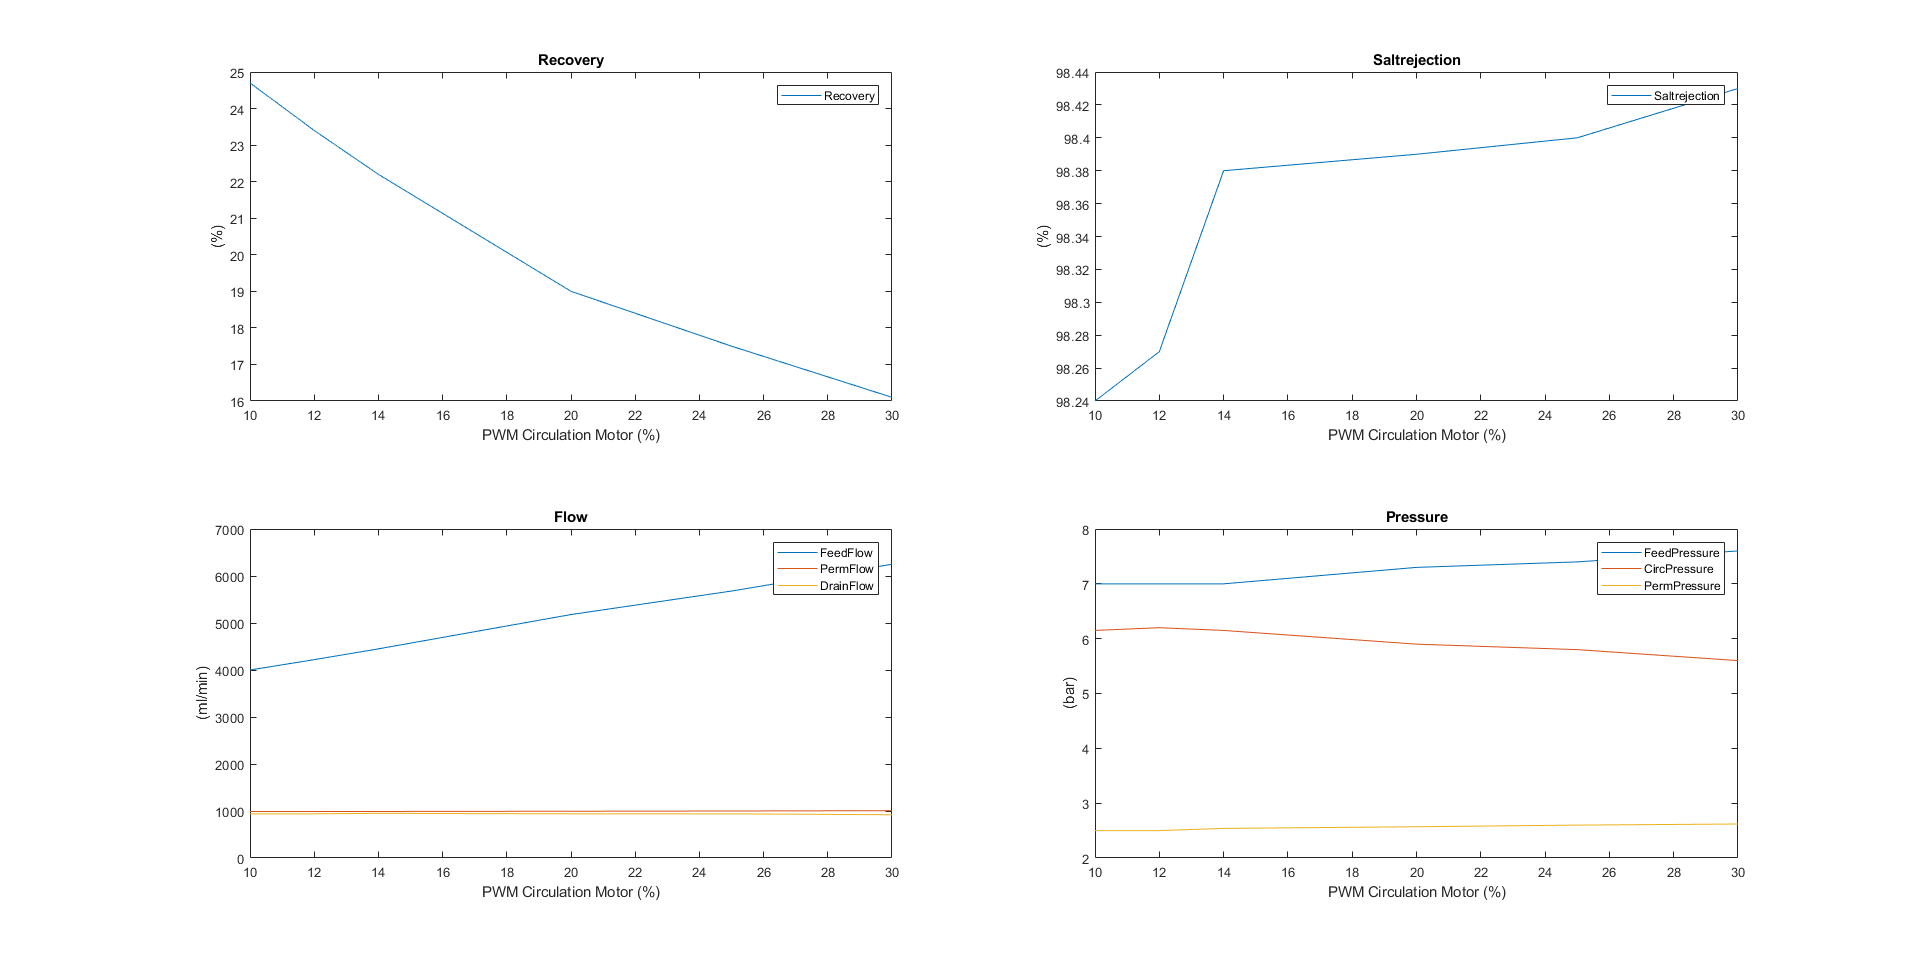
\includegraphics[width=1.65\textwidth, angle = 270]{PreTestReg1.png}
    \caption{Tests with recycle pump as changing parameter}
    \label{fig:PreTestReg1}
\end{figure}

\begin{figure}[h]
    \centering 
    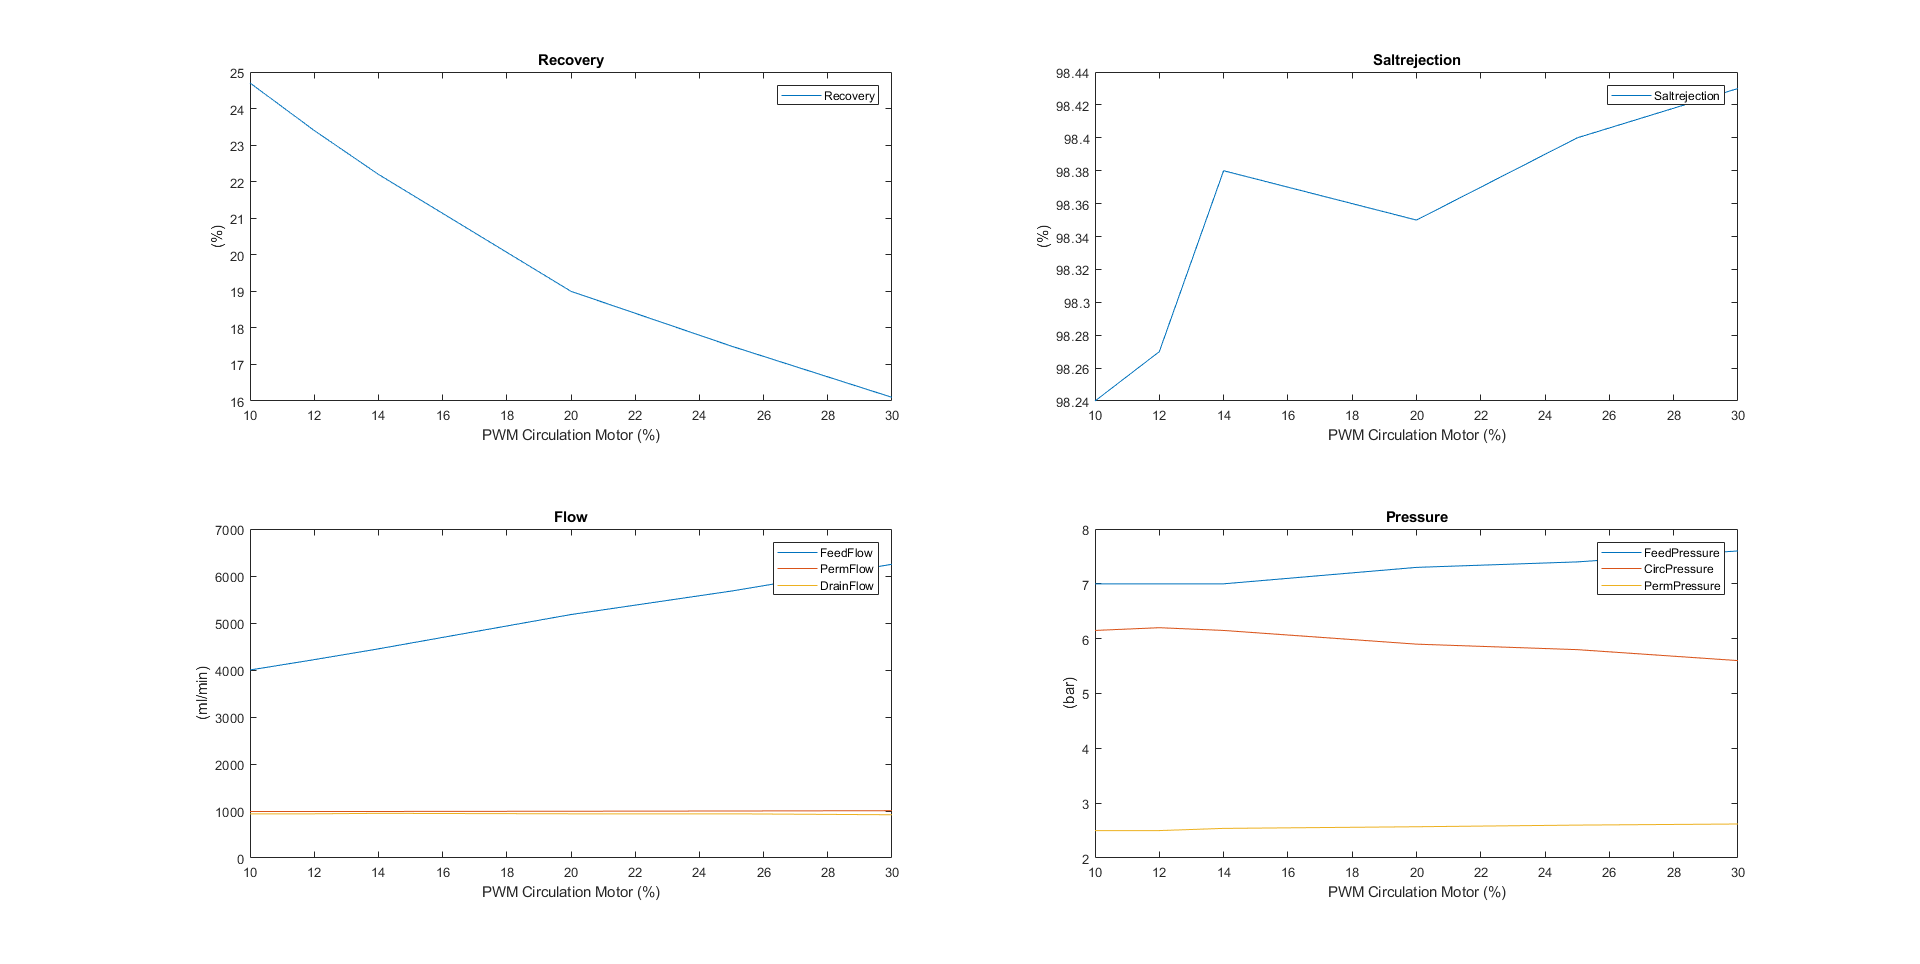
\includegraphics[width=1.65\textwidth, angle=270]{PreTestReg3.png}
    \caption{Tests with inlet pump as changing parameter}
    \label{fig:PreTestReg3}
\end{figure}





